\documentclass{llncs}
\usepackage{makeidx}  
\usepackage{color}
\usepackage{graphicx}
\usepackage{latexsym}
\usepackage{stmaryrd}
\usepackage{amsmath}
\usepackage{amssymb}
\usepackage{stmaryrd}
\usepackage{mathpartir}
\usepackage{wasysym}
\usepackage{booktabs}

\usepackage{courier}            % standard fixed width font
\usepackage[scaled]{helvet} % see www.ctan.org/get/macros/latex/required/psnfss/psnfss2e.pdf

\usepackage{url}             % format URLs

\usepackage{listings}          % format code
\usepackage{enumitem}      % adjust spacing in enums
\usepackage[colorlinks=true,allcolors=blue,breaklinks,draft=false]{hyperref}   % hyperlinks, including DOIs and URLs in bibliography
% known bug: http://tex.stackexchange.com/questions/1522/pdfendlink-ended-up-in-different-nesting-level-than-pdfstartlink
\newcommand{\doi}[1]{doi:~\href{http://dx.doi.org/#1}{\Hurl{#1}}}   % print a hyperlinked DOI
\newcommand{\imageof}[1]{\llbracket #1 \rrbracket}

\usepackage{fancyvrb}
\usepackage{lipsum}
\usepackage{comment}
\usepackage{todonotes}

\usepackage{mathpartir}

\definecolor{light}{gray}{.75}

\lstset{ %
language=Java,                % choose the language of the code
columns=flexible,
lineskip=-1pt,
basicstyle=\ttfamily\small,       % the size of the fonts that are used for the code
numbers=none,                   % where to put the line-numbers
numberstyle=\ttfamily\tiny,      % the size of the fonts that are used for the line-numbers
stepnumber=1,                   % the step between two line-numbers. If it's 1 each line will be numbered
numbersep=5pt,                  % how far the line-numbers are from the code
backgroundcolor=\color{white},  % choose the background color. You must add \usepackage{color}
showspaces=false,               % show spaces adding particular underscores
showstringspaces=false,         % underline spaces within strings
showtabs=false,                 % show tabs within strings adding particular underscores
morekeywords={var},
%  frame=single,                   % adds a frame around the code
tabsize=2,                  % sets default tabsize to 2 spaces
captionpos=none,                   % sets the caption-position to bottom
breaklines=true,                % sets automatic line breaking
breakatwhitespace=false,        % sets if automatic breaks should only happen at whitespace
title=\lstname,                 % show the filename of files included with \lstinputlisting; also try caption instead of title
escapeinside={(*}{*)},          % if you want to add a comment within your code
keywordstyle=\ttfamily\bfseries
}

\newcommand{\gbox}[1]{\colorbox{light}{$\!\!#1\!\!$}}

\newcommand{\name}{{\bf FCore~}}
\newcommand{\Name}{{\bf FCore}}

% General
\newcommand{\code}[1]{\texttt {#1}}
\newcommand{\highlight}[1]{\colorbox{GreenYellow}{#1}}

% Math
\newcommand{\im}[1]{\lvert #1 \rvert}

% Constructors
\newcommand{\for}[2]{\forall #1. \, #2}
\newcommand{\lam}[2]{\lambda #1. \, #2}
\newcommand{\app}[2]{#1 \; #2}
\newcommand{\blam}[2]{\Lambda #1. #2}
\newcommand{\tapp}[2]{#1 \; #2}


\newcommand{\arrow}{\rightarrow}

% \newtheorem{theorem}{Theorem}[section]
% \newtheorem{conjecture}{Conjecture}[section]
% \newtheorem{lemma}{Lemma}[section]
% \newtheorem{definition}{Definition}[section]
% \newtheorem{proposition}[theorem]{Proposition}
% \newtheorem{corollary}[theorem]{Corollary}

\newcommand{\mca}{\mathcal{A}}
\newcommand{\mcb}{\mathcal{B}}
\newcommand{\mcc}{\mathcal{C}}
\newcommand{\mcd}{\mathcal{D}}
\newcommand{\mce}{\mathcal{E}}
\newcommand{\mcf}{\mathcal{F}}
\newcommand{\mcg}{\mathcal{G}}
\newcommand{\mch}{\mathcal{H}}
\newcommand{\mci}{\mathcal{I}}
\newcommand{\mcj}{\mathcal{J}}
\newcommand{\mck}{\mathcal{K}}
\newcommand{\mcl}{\mathcal{L}}
\newcommand{\mcm}{\mathcal{M}}
\newcommand{\mcn}{\mathcal{N}}
\newcommand{\mco}{\mathcal{O}}
\newcommand{\mcp}{\mathcal{P}}
\newcommand{\mcq}{\mathcal{Q}}
\newcommand{\mcr}{\mathcal{R}}
\newcommand{\mcs}{\mathcal{S}}
\newcommand{\mct}{\mathcal{T}}
\newcommand{\mcu}{\mathcal{U}}
\newcommand{\mcv}{\mathcal{V}}
\newcommand{\mcw}{\mathcal{W}}
\newcommand{\mcx}{\mathcal{X}}
\newcommand{\mcy}{\mathcal{Y}}
\newcommand{\mcz}{\mathcal{Z}}

\newcommand{\ourlang}{\lambda_{?}}
\newcommand{\ourpolylang}{\lambda_{\rho}^{\it poly}}

\newcommand{\figtwocol}[3]
{\begin{figure}[h!] #3 \caption{#2}\label{#1}\end{figure}}

\newcommand{\myirule}[2]{{\renewcommand{\arraystretch}{1.2}\ba{c} #1
                      \\ \hline #2 \ea}}

\newcommand{\ba}{\begin{array}}
\newcommand{\ea}{\end{array}}
\newcommand{\bda}{\[\ba}
\newcommand{\eda}{\ea\]}

\newcommand{\myset}[1]{\{#1\}}
\newcommand{\relation}[2]{#1:#2}
\newcommand{\myrelation}[2]{#1\!:\!#2}
\newcommand{\To}{\Rightarrow}

\newcommand{\Abs}[2]{\Lambda #1. #2}
\newcommand{\abs}[2]{\lambda #1. #2}
%\newcommand{\ruleabs}[2]{\langle\!|  #2  :  #1 |\!\rangle}
%\newcommand{\ruleabs}[2]{(\!|  #2  :  #1 |\!)}
\newcommand{\ruleabs}[2]{\lambda_? #1. #2}
\newcommand{\ruleapp}[2]{#1 {\bf ~with~} #2}
\newcommand{\iarrow}{\Rightarrow}
\newcommand{\ilambda}{\lambda_{?}}
\newcommand{\with}{{\bf ~with~}}
\newcommand{\query}{?}
\newcommand{\type}{\tau}
\newcommand{\tyint}{{\it Int}}
\newcommand{\tybool}{{\it Bool}}
\newcommand{\tychar}{{\it Char}}
\newcommand{\tystr}{{\it String}}
\newcommand{\tyunit}{()}
\newcommand{\unit}{()}
\newcommand{\btrue}{{\it True}}
\newcommand{\bfalse}{{\it False}}
\newcommand{\Eq}{{\tt Eq}}
\newcommand{\ShowC}{{\tt ShowC}}
\newcommand{\Monad}{{\tt Monad}}
\newcommand{\MonadTrans}{{\tt MonadTrans}}
\newcommand{\GTree}{{\tt GTree}}
\newcommand{\TT}{{\tt \#t}}
\newcommand{\FF}{{\tt \#f}}


\newcommand{\kind}{\kappa}
\newcommand{\rulet}{\rho}
\newcommand{\ruleschr}[3]
{\forall #1. #2 \To #3}
\newcommand{\rulesch}[3]
{\forall \vec{#1}. #2 \To #3}
\newcommand{\ruleset}{\bar{\rulet}}
\newcommand{\rulesetvar}{\ruleset}
\newcommand{\nil}{\varnothing}
\newcommand{\meta}[1]{{\it #1 }}
\newcommand{\finto}{\stackrel{\mathsf{fin}}{\to}}
\newcommand{\rulepgm}{\overline{\relation{\rulet}{v}}}
\newcommand{\rulepgmvar}{\eta}
\newcommand{\grulepgm}[2]{\overline{\relation{#1}{#2}}}
\newcommand{\rulesetexp}{\overline{\relation{e}{\rulet}}}

\newcommand{\FV}     {\meta{fv}}
\newcommand{\FTV}    {\meta{FTV}}
\newcommand{\BV}     {\meta{bv}}
\newcommand{\BTV}    {\meta{BTV}}
\newcommand{\dom}    {\meta{dom}}

\newcommand{\tstate}{\mce}
\newcommand{\rclos}[1]{(#1)}
\newcommand{\lookup}[2]{{#1\langle{#2}\rangle}}
\newcommand{\kenv}{\Phi}
\newcommand{\denv}{\Delta}
\newcommand{\env}{\Delta}
\newcommand{\tenv}{\Gamma}
\newcommand{\eval}{\Downarrow}
\newcommand{\turns}{\vdash}
\newcommand{\vturns}{\vdash_{r}}
\newcommand{\kturns}{\vdash_{k}}
\newcommand{\vtyping}{\models}

%\newcommand{\case}[1]{\----{\bf case}~#1}
\newcommand{\facerule}[1]{{\tt #1}}
\newcommand{\tlabel}[1]{\mbox{(#1)}}

\newcommand{\mylabel}[1]{\tlabel{\facerule{#1}}}

\newcommand{\OpQuery}{\tlabel{\facerule{OpQuery}}}
\newcommand{\OpRule}{\tlabel{\facerule{OpRule}}}
\newcommand{\OpInst}{\tlabel{\facerule{OpInst}}}
\newcommand{\OpRApp}{\tlabel{\facerule{OpRApp}}}
\newcommand{\OpRClos}{\tlabel{\facerule{OpRClos}}}

\newcommand{\TyQuery}{\tlabel{\facerule{Ty-Query}}}
\newcommand{\TyRule}{\tlabel{\facerule{TyRule}}}
\newcommand{\TyInst}{\tlabel{\facerule{TyInst}}}
\newcommand{\TyRApp}{\tlabel{\facerule{TyRApp}}}

\newcommand{\TyRClos}{\tlabel{\facerule{TyRClos}}}
\newcommand{\TyREnv}{\tlabel{\facerule{TyREnv}}}
\newcommand{\TyRPgm}{\tlabel{\facerule{TyRPgm}}}

\newcommand{\RTAbs}{\tlabel{\facerule{RTAbs}}}
\newcommand{\RIAbs}{\tlabel{\facerule{RIAbs}}}
\newcommand{\RSimpl}{\tlabel{\facerule{RSimp}}}

\newcommand{\IDone}{\tlabel{\facerule{IDone}}}
\newcommand{\ITAbs}{\tlabel{\facerule{ITAbs}}}
\newcommand{\IIAbs}{\tlabel{\facerule{IIAbs}}}

\newcommand{\LHere}{\tlabel{\facerule{LHead}}}
\newcommand{\LThere}{\tlabel{\facerule{LTail}}}

\newcommand{\MDone}{\tlabel{\facerule{MDone}}}
\newcommand{\MTAbs}{\tlabel{\facerule{MTAbs}}}
\newcommand{\MIAbs}{\tlabel{\facerule{MIAbs}}}

\newcommand{\TrRTAbs}{\tlabel{\facerule{TrRTAbs}}}
\newcommand{\RRho}{\tlabel{\facerule{RRho}}}
\newcommand{\TrRIAbs}{\tlabel{\facerule{TrRIAbs}}}
\newcommand{\TrRSimpl}{\tlabel{\facerule{TrRSimp}}}

\newcommand{\TrIDone}{\tlabel{\facerule{TrIDone}}}
\newcommand{\TrITAbs}{\tlabel{\facerule{TrITAbs}}}
\newcommand{\TrIIAbs}{\tlabel{\facerule{TrIIAbs}}}

\newcommand{\TrLHere}{\tlabel{\facerule{TrLHead}}}
\newcommand{\TrLThere}{\tlabel{\facerule{TrLTail}}}


\newcommand{\TrInt}{\tlabel{\facerule{TrInt}}}
\newcommand{\TrVar}{\tlabel{\facerule{TrVar}}}
\newcommand{\TrAbs}{\tlabel{\facerule{TrAbs}}}
\newcommand{\TrApp}{\tlabel{\facerule{TrApp}}}
\newcommand{\TrTAbs}{\tlabel{\facerule{TrTAbs}}}
\newcommand{\TrTApp}{\tlabel{\facerule{TrTApp}}}
\newcommand{\TrIAbs}{\tlabel{\facerule{TrIAbs}}}
\newcommand{\TrIApp}{\tlabel{\facerule{TrIApp}}}
\newcommand{\TrQuery}{\tlabel{\facerule{TrQuery}}}

\newcommand{\TermSimpl}{\tlabel{\facerule{TermSimp}}}
\newcommand{\TermTyVar}{\tlabel{\facerule{TermTyVar}}}
\newcommand{\TermInt}{\tlabel{\facerule{TermInt}}}
\newcommand{\TermForall}{\tlabel{\facerule{TermForall}}}
\newcommand{\TermFun}{\tlabel{\facerule{TermFun}}}
\newcommand{\TermRule}{\tlabel{\facerule{TermRule}}}

\newcommand{\ResNil}{\tlabel{\facerule{ResNil}}}
\newcommand{\Res}{\tlabel{\facerule{Res}}}
\newcommand{\SimpleRes}{\tlabel{\facerule{SimpleRes}}}
\newcommand{\RuleRes}{\tlabel{\facerule{RuleRes}}}
\newcommand{\StaRes}{\tlabel{\facerule{TyRes}}}
\newcommand{\DynRes}{\tlabel{\facerule{DynRes}}}

\newcommand{\TrRes}{\tlabel{\facerule{TrRes}}}

\newcommand{\Canon}[1]{\mathsf{canon}(#1)}
\newcommand{\unify}[3]{\mcu_{#3}(#1, #2)}

\newcommand{\KiVar}{\tlabel{\facerule{KiVar}}}
\newcommand{\KiApp}{\tlabel{\facerule{KiApp}}}
\newcommand{\KiForall}{\tlabel{\facerule{KiForall}}}

\newcommand{\err}{{\it err}}

\def\ruleform#1{{\setlength{\fboxrule}{1pt}\fbox{\normalsize $#1$}}}

\newcommand{\Ex}[1]{\[\begin{array}{l}#1\end{array}\]}
\newcommand{\Cmnt}[1]{{\tt #1}}

\newcommand{\subst}[2]{[ #1\!\mapsto\!#2 ]}
\newcommand{\substone}{\subst{\alpha}{\type}}

\newcommand{\leteq}{\overset{{\sf let}}{=}}
\newcommand{\defeq}{\overset{{\sf def}}{=}}

\newcommand{\overlap}{{\sf overlap}}
\newcommand{\nonoverlap}{{\sf nonoverlap}}
\newcommand{\wellformed}{{\sf wellformed}}
\newcommand{\stable}{{\sf stable}}
\newcommand{\coherent}{{\sf coherent}}
\newcommand{\distinct}{{\sf distinct}}
\newcommand{\unrelated}{{\sf unrelated}}
\newcommand{\disjoint}{{\sf distinct}}
\newcommand{\converge}{{\sf converge}}
\newcommand{\welldefined}{{\sf welldefined}}

\newcommand{\distinctrs}{{\sf distinct\_rs}}
\newcommand{\distinctctx}{{\sf distinct\_ctx}}
\newcommand{\distinctwith}{{\sf distinct\_with}}
\newcommand{\unambiguous}{{\sf unambiguous}}

\definecolor{gray}{gray}{0.7}
\definecolor{dark-gray}{gray}{0.4}
\definecolor{light-gray}{gray}{0.8}

%\newcommand{\shade}[1]{\colorbox{gray}{\color{dark-gray} {$#1$}}}
%\newcommand{\shade}[1]{\colorbox{light-gray}{\color{dark-gray} {$#1$}}}
\newcommand{\shade}[1]{\colorbox{light-gray}{\color{black}{$#1$}}}
\newcommand{\hide}[1]{}
\def\myruleform#1{
\setlength{\fboxrule}{0.5pt}\fbox{\normalsize $#1$}
}

\newcommand{\WFIntTy}{\tlabel{\facerule{WF-IntTy}}}
\newcommand{\WFVarTy}{\tlabel{\facerule{WF-VarTy}}}
\newcommand{\WFAbsTy}{\tlabel{\facerule{WF-AbsTy}}}
\newcommand{\WFFunTy}{\tlabel{\facerule{WF-FunTy}}}
\newcommand{\WFRulTy}{\tlabel{\facerule{WF-RulTy}}}

\newcommand{\TyTyAbs}{\tlabel{\facerule{TyTyAbs}}}
\newcommand{\TyTyApp}{\tlabel{\facerule{TyTyApp}}}
\newcommand{\TyUnit}{\tlabel{\facerule{TyUnit}}}
\newcommand{\TyInt}{\tlabel{\facerule{Ty-Int}}}
\newcommand{\TyVar}{\tlabel{\facerule{Ty-Var}}}
\newcommand{\TyIntL}{\tlabel{\facerule{TyIntL}}}
\newcommand{\TyLVar}{\tlabel{\facerule{TyLVar}}}
\newcommand{\TyIVar}{\tlabel{\facerule{TyIVar}}}
\newcommand{\TyRec}{\tlabel{\facerule{TyRec}}}
\newcommand{\TyAbs}{\tlabel{\facerule{Ty-Abs}}}
\newcommand{\TyTAbs}{\tlabel{\facerule{Ty-TAbs}}}
\newcommand{\TyIAbs}{\tlabel{\facerule{Ty-IAbs}}}
\newcommand{\TyApp}{\tlabel{\facerule{Ty-App}}}
\newcommand{\TyTApp}{\tlabel{\facerule{Ty-TApp}}}
\newcommand{\TyIApp}{\tlabel{\facerule{Ty-IApp}}}
\newcommand{\TyLet}{\tlabel{\facerule{TyLet}}}
\newcommand{\TyImp}{\tlabel{\facerule{TyImp}}}
\newcommand{\TyWith}{\tlabel{\facerule{TyWith}}}
\newcommand{\TyAnn}{\tlabel{\facerule{TyAnn}}}

\newcommand{\eqv}{\Longleftrightarrow}

%%% Local Variables: 
%%% mode: latex
%%% TeX-master: "Main"
%%% End: 

%%include lhs2TeX.fmt
%% ODER: format ==         = "\mathrel{==}"
%% ODER: format /=         = "\neq "
%
%
\makeatletter
\@ifundefined{lhs2tex.lhs2tex.sty.read}%
  {\@namedef{lhs2tex.lhs2tex.sty.read}{}%
   \newcommand\SkipToFmtEnd{}%
   \newcommand\EndFmtInput{}%
   \long\def\SkipToFmtEnd#1\EndFmtInput{}%
  }\SkipToFmtEnd

\newcommand\ReadOnlyOnce[1]{\@ifundefined{#1}{\@namedef{#1}{}}\SkipToFmtEnd}
\usepackage{amstext}
\usepackage{amssymb}
\usepackage{stmaryrd}
\DeclareFontFamily{OT1}{cmtex}{}
\DeclareFontShape{OT1}{cmtex}{m}{n}
  {<5><6><7><8>cmtex8
   <9>cmtex9
   <10><10.95><12><14.4><17.28><20.74><24.88>cmtex10}{}
\DeclareFontShape{OT1}{cmtex}{m}{it}
  {<-> ssub * cmtt/m/it}{}
\newcommand{\texfamily}{\fontfamily{cmtex}\selectfont}
\DeclareFontShape{OT1}{cmtt}{bx}{n}
  {<5><6><7><8>cmtt8
   <9>cmbtt9
   <10><10.95><12><14.4><17.28><20.74><24.88>cmbtt10}{}
\DeclareFontShape{OT1}{cmtex}{bx}{n}
  {<-> ssub * cmtt/bx/n}{}
\newcommand{\tex}[1]{\text{\texfamily#1}}	% NEU

\newcommand{\Sp}{\hskip.33334em\relax}


\newcommand{\Conid}[1]{\mathit{#1}}
\newcommand{\Varid}[1]{\mathit{#1}}
\newcommand{\anonymous}{\kern0.06em \vbox{\hrule\@width.5em}}
\newcommand{\plus}{\mathbin{+\!\!\!+}}
\newcommand{\bind}{\mathbin{>\!\!\!>\mkern-6.7mu=}}
\newcommand{\rbind}{\mathbin{=\mkern-6.7mu<\!\!\!<}}% suggested by Neil Mitchell
\newcommand{\sequ}{\mathbin{>\!\!\!>}}
\renewcommand{\leq}{\leqslant}
\renewcommand{\geq}{\geqslant}
\usepackage{polytable}

%mathindent has to be defined
\@ifundefined{mathindent}%
  {\newdimen\mathindent\mathindent\leftmargini}%
  {}%

\def\resethooks{%
  \global\let\SaveRestoreHook\empty
  \global\let\ColumnHook\empty}
\newcommand*{\savecolumns}[1][default]%
  {\g@addto@macro\SaveRestoreHook{\savecolumns[#1]}}
\newcommand*{\restorecolumns}[1][default]%
  {\g@addto@macro\SaveRestoreHook{\restorecolumns[#1]}}
\newcommand*{\aligncolumn}[2]%
  {\g@addto@macro\ColumnHook{\column{#1}{#2}}}

\resethooks

\newcommand{\onelinecommentchars}{\quad-{}- }
\newcommand{\commentbeginchars}{\enskip\{-}
\newcommand{\commentendchars}{-\}\enskip}

\newcommand{\visiblecomments}{%
  \let\onelinecomment=\onelinecommentchars
  \let\commentbegin=\commentbeginchars
  \let\commentend=\commentendchars}

\newcommand{\invisiblecomments}{%
  \let\onelinecomment=\empty
  \let\commentbegin=\empty
  \let\commentend=\empty}

\visiblecomments

\newlength{\blanklineskip}
\setlength{\blanklineskip}{0.66084ex}

\newcommand{\hsindent}[1]{\quad}% default is fixed indentation
\let\hspre\empty
\let\hspost\empty
\newcommand{\NB}{\textbf{NB}}
\newcommand{\Todo}[1]{$\langle$\textbf{To do:}~#1$\rangle$}

\EndFmtInput
\makeatother
%
%
%
%
%
%
% This package provides two environments suitable to take the place
% of hscode, called "plainhscode" and "arrayhscode". 
%
% The plain environment surrounds each code block by vertical space,
% and it uses \abovedisplayskip and \belowdisplayskip to get spacing
% similar to formulas. Note that if these dimensions are changed,
% the spacing around displayed math formulas changes as well.
% All code is indented using \leftskip.
%
% Changed 19.08.2004 to reflect changes in colorcode. Should work with
% CodeGroup.sty.
%
\ReadOnlyOnce{polycode.fmt}%
\makeatletter

\newcommand{\hsnewpar}[1]%
  {{\parskip=0pt\parindent=0pt\par\vskip #1\noindent}}

% can be used, for instance, to redefine the code size, by setting the
% command to \small or something alike
\newcommand{\hscodestyle}{}

% The command \sethscode can be used to switch the code formatting
% behaviour by mapping the hscode environment in the subst directive
% to a new LaTeX environment.

\newcommand{\sethscode}[1]%
  {\expandafter\let\expandafter\hscode\csname #1\endcsname
   \expandafter\let\expandafter\endhscode\csname end#1\endcsname}

% "compatibility" mode restores the non-polycode.fmt layout.

\newenvironment{compathscode}%
  {\par\noindent
   \advance\leftskip\mathindent
   \hscodestyle
   \let\\=\@normalcr
   \(\pboxed}%
  {\endpboxed\)%
   \par\noindent
   \ignorespacesafterend}

\newcommand{\compaths}{\sethscode{compathscode}}

% "plain" mode is the proposed default.

\newenvironment{plainhscode}%
  {\hsnewpar\abovedisplayskip
   \advance\leftskip\mathindent
   \hscodestyle
   \let\\=\@normalcr
   \(\pboxed}%
  {\endpboxed\)%
   \hsnewpar\belowdisplayskip
   \ignorespacesafterend}

% Here, we make plainhscode the default environment.

\newcommand{\plainhs}{\sethscode{plainhscode}}
\plainhs

% The arrayhscode is like plain, but makes use of polytable's
% parray environment which disallows page breaks in code blocks.

\newenvironment{arrayhscode}%
  {\hsnewpar\abovedisplayskip
   \advance\leftskip\mathindent
   \hscodestyle
   \let\\=\@normalcr
   \(\parray}%
  {\endparray\)%
   \hsnewpar\belowdisplayskip
   \ignorespacesafterend}

\newcommand{\arrayhs}{\sethscode{arrayhscode}}

% The mathhscode environment also makes use of polytable's parray 
% environment. It is supposed to be used only inside math mode 
% (I used it to typeset the type rules in my thesis).

\newenvironment{mathhscode}%
  {\parray}{\endparray}

\newcommand{\mathhs}{\sethscode{mathhscode}}

% texths is similar to mathhs, but works in text mode.

\newenvironment{texthscode}%
  {\(\parray}{\endparray\)}

\newcommand{\texths}{\sethscode{texthscode}}

% The framed environment places code in a framed box.

\def\codeframewidth{\arrayrulewidth}
\RequirePackage{calc}

\newenvironment{framedhscode}%
  {\parskip=\abovedisplayskip\par\noindent
   \hscodestyle
   \arrayrulewidth=\codeframewidth
   \tabular{@{}|p{\linewidth-2\arraycolsep-2\arrayrulewidth-2pt}|@{}}%
   \hline\framedhslinecorrect\\{-1.5ex}%
   \let\endoflinesave=\\
   \let\\=\@normalcr
   \(\pboxed}%
  {\endpboxed\)%
   \framedhslinecorrect\endoflinesave{.5ex}\hline
   \endtabular
   \parskip=\belowdisplayskip\par\noindent
   \ignorespacesafterend}

\newcommand{\framedhslinecorrect}[2]%
  {#1[#2]}

\newcommand{\framedhs}{\sethscode{framedhscode}}

% The inlinehscode environment is an experimental environment
% that can be used to typeset displayed code inline.

\newenvironment{inlinehscode}%
  {\(\def\column##1##2{}%
   \let\>\undefined\let\<\undefined\let\\\undefined
   \newcommand\>[1][]{}\newcommand\<[1][]{}\newcommand\\[1][]{}%
   \def\fromto##1##2##3{##3}%
   \def\nextline{}}{\) }%

\newcommand{\inlinehs}{\sethscode{inlinehscode}}

% The joincode environment is a separate environment that
% can be used to surround and thereby connect multiple code
% blocks.

\newenvironment{joincode}%
  {\let\orighscode=\hscode
   \let\origendhscode=\endhscode
   \def\endhscode{\def\hscode{\endgroup\def\@currenvir{hscode}\\}\begingroup}
   %\let\SaveRestoreHook=\empty
   %\let\ColumnHook=\empty
   %\let\resethooks=\empty
   \orighscode\def\hscode{\endgroup\def\@currenvir{hscode}}}%
  {\origendhscode
   \global\let\hscode=\orighscode
   \global\let\endhscode=\origendhscode}%

\makeatother
\EndFmtInput
%

% Document starts
\begin{document}

\lstset{keywordstyle=\textbf,language=Java}

\title{Memory-efficient Tail Calls in the JVM with Imperative Functional Objects}

\author{Tom\'{a}\v{s} Tauber\inst{1}, Xuan Bi\inst{1}, Zhiyuan Shi\inst{1},
Weixin Zhang\inst{1}, Huang Li\inst{2}, Zhenrui Zhang\inst{2}, Bruno C. d. S. Oliveira\inst{1}}
%
\authorrunning{Tom\'{a}\v{s} Tauber et al.} 
\tocauthor{Tom\'{a}\v{s} Tauber, Xuan Bi, Zhiyuan Shi,
Weixin Zhang, Huang Li, Zhenrui Zhang, Bruno C. d. S. Oliveira}
%
\institute{The University of Hong Kong, Pok Fu Lam Road, Hong Kong SAR 
\and
Zhejiang University, 38 Zheda Road, Hangzhou, China}

\maketitle

\begin{abstract}

This paper presents \Name: a JVM implementation of System F
with support for full \emph{tail-call elimination} (TCE). 
Our compilation technique for \name is innovative in two respects: it
uses a new representation for first-class functions called
\emph{imperative functional objects}; and it provides a way
to do TCE on the JVM using constant space.

Unlike conventional TCE techniques on the JVM, allocated function objects
are reused in chains of tail calls.
Thus, programs written in \name
can use idiomatic functional programming styles, relying
on TCE, and perform well without worrying about
the JVM limitations. Our empirical results show that programs which use tail calls
can run in constant space and with low execution time overhead when compiled with \Name.

\end{abstract}

\section{Introduction}\label{sec:intro}

% Motivation
A runtime environment, such as the JVM, attracts both functional programming (FP) languages'
compiler writers and users: it enables cross-platform development and comes with a
large collection of libraries and tools. Moreover, FP languages give programmers
on the JVM other benefits: simple, concise and elegant ways to write different algorithms;
high code reuse via higher-order functions; and more opportunities for parallelism,
 by avoiding the overuse of side-effects (and shared mutable state) \cite{erlang}.
 Unfortunately, compilers for functional languages are hard to
implement efficiently in the JVM. FP promotes a
programming style where \emph{functions are first-class values} and \emph{recursion} is used
instead of mutable state and loops to define algorithms. The JVM is
not designed to deal with such programs.


The difficulty in optimizing FP in the JVM means that:
\emph{while FP in the JVM is possible today,
some compromises are still necessary for writing efficient programs.}
Existing JVM functional languages, including
Scala~\cite{Odersky2014b}
and Clojure~\cite{Hickey2008}, usually
work around the challenges imposed by the JVM. Those languages give
programmers alternatives to a FP
style. Therefore, performance-aware programmers avoid certain idiomatic
FP styles, which may be costly in those languages, and use
the available alternatives instead.

%\paragraph{JVM Challenges}
In particular, one infamous challenge when writing a
compiler for a functional language targeting the JVM is: How to eliminate and/or optimize tail calls?
Before tackling that, one needs to decide how to represent functions in the JVM.
There are two standard options: \emph{JVM methods} and
\emph{functions as objects} (FAOs).
Encoding first-class functions using only JVM methods directly is
limiting: JVM methods cannot encode currying and partial function application directly.
To support these features, the majority of functional languages or extensions (including Scala,
Clojure, and Java 8) adopt variants of the functions-as-objects
approach:

\begin{lstlisting}
interface FAO { Object apply(Object arg);}
\end{lstlisting}

\noindent With this representation,
we can encode curried functions, partial application and
pass functions as arguments.
However, neither FAOs nor JVM methods offer a good solution to
deal with \emph{general tail-call elimination}
(TCE)~\cite{Steele1977}. The JVM does not support proper tail calls.
In particular scenarios, such as single, tail-recursive calls, we can
easily achieve an optimal solution in the JVM.  Both Scala and Clojure
provide some support for tail-recursion~\cite{Odersky2014b,recur}.
However, for more general tail calls (such as mutually recursive
functions or non-recursive tail calls), existing solutions can worsen
the overall performance. For example, JVM-style trampolines~\cite{Schinz2001}
(which provide a general solution for tail calls) are significantly
slower than normal calls and consume heap memory for every tail call.

\subsubsection{Contributions.}
This paper presents a new JVM compilation technique for
functional programs, and creates an implementation of System
F~\cite{girard72dissertation,reynolds74towards} using the new
technique. The compilation technique builds on a new representation of
first-class functions in the JVM: \emph{imperative functional
  objects} (IFOs).
\emph{With IFOs it is possible to use a single
 representation of functions in the JVM and still achieve memory-efficient TCE}.
 As a first-class function representation, IFOs also support currying and
 partial function applications.

We represent an IFO by the following abstract class:

\begin{lstlisting}
abstract class Function {
   Object arg, res;
   abstract void apply();
}
\end{lstlisting}

\noindent With IFOs, we encode both the argument
(\lstinline{arg}) and the result of the functions (\lstinline{res})
as mutable fields.
We set the argument field before
invoking the \lstinline{apply()} method. At the end of the \lstinline{apply()} method, we set  the result field.
An important difference between the IFOs and FAOs encoding of
first-class functions is that, in IFOs, \emph{function application is
divided in two parts}: \emph{setting the argument field}; and \emph{invoking the
apply method}.
For example, if we have a function call
\lstinline{factorial 10}, the corresponding Java code using IFOs
is:

\begin{lstlisting}
factorial.arg = 10;  // setting argument
factorial.apply();      // invoking function
\end{lstlisting}

The fact that we can split function application into two parts is key
to enable new optimizations related to functions
in the JVM. In particular, the TCE
approach with IFOs does not require memory allocation for each tail
call and has less execution time overhead than the JVM-style trampolines used in languages
such as Clojure and Scala. Essentially, with IFOs, it is possible to
provide a straightforward TCE implementation, resembling Steele's ``UUO
handler''~\cite{Steele1978}, in the JVM.

Using IFOs and the TCE technique, we created
\Name: a JVM implementation of an extension of \emph{System
  F}.
\name aims to serve as an intermediate functional layer on top
of the JVM, which ML-style languages can target. According to our experimental results,
\name programs perform competitively against programs using regular JVM methods,
while still supporting TCE. Programs in \name tend to have
less execution time overhead
and use less memory than programs using conventional
JVM trampolines.

In summary, the contributions of this paper are:

\begin{itemize}

\item {\bf Imperative Functional Objects:} A new representation of
  first-class functions in the JVM, offering new ways to
  optimize functional programs.

\item {\bf A memory-efficient approach to tail-call elimination:} A way to
  implement TCE in the JVM using IFOs without allocating memory per each tail call.

\item \Name: An implementation of a System F-based
  intermediate language that can be used to target the JVM by FP
  compilers.

\item {\bf Formalization and empirical results:} Our basic compilation
  method from a subset of \name into Java is formalized. Our empirical
  results indicate that \name allows general TCE in constant memory space
  and with execution time comparable to regular JVM methods.

\end{itemize}




\section{\name and IFOs, Informally}\label{sec:overview}

This section informally presents \name programs and their IFO-based
encoding. It also shows how to deal with tail-call elimination.
Sections~\ref{sec:fcore} and \ref{sec:tce} present a formalized
compilation method for a subset of \name (System F) into Middleweight Java, 
a formalized subset of Java, based on the ideas from this section.
Note that, for purposes of presentation, we simplify the encodings shown in this
section slightly compared to what we generate by our formal compilation
method.


\begin{comment}
\subsection{Imperative Functional Objects}

\begin{figure}[t]

% use scala
\begin{lstlisting}
def tfact : Int => Int => Int = acc => n => 
  if (n == 0) acc else tfact(acc*n)(n-1)

def even : Int => Boolean = n =>
    if (n == 0) true else odd(n-1)
    
def odd : Int => Boolean = n =>
    if (n == 0) false else even(n-1)
\end{lstlisting}

\caption{Scala function definitions for computing factorial, even and odd.}

\label{fig:scala_defs}

\end{figure}

Currently, functional programming in the JVM requires some compromises, especially 
when performance or memory are primary considerations. For example, consider the 
Scala functions in Figure~\ref{fig:scala_defs}.
The function \lstinline{tfact} computes the factorial of some number
\lstinline{n} using a standard tail-recursive implementation with an accumulator.  The
functions \lstinline{even} and \lstinline{odd} define a naive
algorithm for detecting whether a number is even or
odd. We define the later two functions using \emph{mutually recursive tail calls}. 
The code uses Scala first-class functions (\lstinline{A => B}), represented by the following trait:
%\footnote{For the purposes of this
%  paper a trait can be interpreted as a Java interface.}:

\begin{lstlisting}
// slightly simplified for presentation
trait Function[A,B] { 
  def apply(x : A) : B
}
\end{lstlisting}

\noindent This trait is a variant of FAOs. A small differerence to 
the \lstinline{FAO} interface presented in Section~\ref{sec:intro}
is that the argument and returned values are typed.
Scala provides a syntactic sugar that makes defining and
applying functions much more convenient than using the
\lstinline{Function} interface directly. The type \lstinline{Int =>Int=> Int} 
corresponds to
\lstinline{Function[Int,Function[Int,Int]]}. In other words, a function
such as \lstinline{tfact} is a function that returns another function. 

%In the code, the function
%\lstinline{tfact} provides a simple recursive implementation of the
%factorial function using an accumulator parameter. Thus computing the
%factorial of a number amounts to calling \lstinline{tfact(0)}. 

While the definitions of the functions in Figure~\ref{fig:scala_defs}
are standard in ML-like languages, they pose problems
in Scala. 

\noindent {\bf Problem 1: Multiple representations of functions} 
The first problem is that, when efficiency is a concern, we need multiple
function representations. JVM
methods are typically a better choice to achieve
performance. Nevertheless, functions as objects are still needed to encode currying
and partial application. 
We can illustrate the performance problem with the definition of
\lstinline{tfact}. In \lstinline{tfact}, every recursive call creates
one new instance of \lstinline{Function} (to encode the second
argument of the function). 

Naive encoding using \lstinline{Function} objects to represent multi-argument
recursive functions can be inefficient. We require an amount of
memory proportional to the number of recursive calls; allocating and
garbage collecting \lstinline{Function} objects incurs a
performance penalty; and invoking methods for each
\lstinline{Function} object adds extra performance penalties.

Alternatively, Scala programmers can use standard 
JVM methods to define \lstinline{tfact}:

\begin{lstlisting}
def tfact2(acc : Int, n : Int) = acc => n => 
  if (n == 0) acc else tfact(acc*n,n-1)
\end{lstlisting}

\noindent This definition is more efficient than 
the one using functions as objects. Indeed in Scala, this is
probably the recommended way to define \lstinline{tfact}. 
However, if we needed to compute, for
example, a list of factorial numbers up to \lstinline{n}, a simple 
functional definition would be:

\begin{lstlisting}
 def facts(n : Int) : List[Int] = 
    List.range(0,n,(x : Int) => x + 1)
      .map(tfact(1))
\end{lstlisting}

\noindent Unfortunately, this definition would not work if we replaced 
\lstinline{tfact} with \lstinline{tfact2}. JVM methods cannot be curried.
Thus to achieve the same effect, we need to change the argument 
of \lstinline{map} to \lstinline{x => tfact(1,x)}, using a functional
object to encode the partial application. 


At the very best, compilers need to be aware of the two possible
representations and try to automatically choose the best representation
for a particular definition or expression. However, it may be
difficult to automatically choose the best representation, since it
depends on how we use the functions. Furthermore, the compilation
process becomes more complicated. 
Some languages, such as Scala,
avoid this problem by offering programmers control over which function
representation to use. However, this makes programming less
transparent: the user now has to decide which representation to
use; and programmers also need to explicitly convert between
these representations. Furthermore, it also makes the language itself 
more complex, since the language constructs that deal 
with we need both representations.



\noindent {\bf Problem 2: Eliminating general tail-calls efficiently
  on the JVM is hard.} We expose the second problem by
\lstinline{even} and \lstinline{odd}. When we call these functions 
on large inputs (typically larger than 10000), the JVM throws a
\lstinline{StackOverflow} exception. In a functional language, we might 
hope that tail-call elimination would prevent \lstinline{StackOverflow}
exceptions and allow tail calls on arbitrarily large
inputs. Unfortunately, the JVM does not provide support for proper 
tail-calls and eliminating tail-calls via other techniques is hard. 
Existing techniques can only deal with direct tail-recursive calls (such as \lstinline{tfact}) effectively on the JVM. However, this excludes 
other classes of useful tail-call functions, including
mutually tail-recursive functions such as \lstinline{even} and \lstinline{odd}.
Although there are some techniques for dealing with general tail calls
in the JVM, these solutions come with important drawbacks. 
For example, trampolines~\cite{} (which provide a general
solution for tail-calls in the JVM) require more time and
memory. Programs using trampolines are usually orders of magnitude times slower
than programs without trampolines.

Generally speaking, tail-call elimination/optimization is essential
for functional programming, for three reasons:

\begin{itemize}

\item {\bf Correctness:} (Proper) tail-call elimination enables programs with tail calls and 
deep call stacks to run without stack overflows. Therefore, 
those programs can terminate normally, instead of with exceptional
behavior.

\item {\bf Space optimization:} (Proper) tail-call elimination removes tail
  calls and removes all stack-space required by these
  calls. Therefore, in contrast to regular calls, tail-calls consume no
  memory.

\item {\bf Time optimization:} When we replace tail calls with jumps, 
the performance of programs greatly improves. Steele's famous 
paper introducing tail call optimization~\cite{Steele1977} illustrated how purely
functional programs written in a functional language can beat
imperative programs written in Fortran using tail-call optimization.

\end{itemize}


The absence of an effective technique for dealing with tail-call
elimination in the JVM means that idiomatic functional programs
have to be rewritten in a different style to achieve correctness and performance.

\end{comment}

\begin{comment}
If we try to compute the
factorial of \lstinline{n}, we need to create \lstinline{n}
\lstinline{Function} objects. Moreover, invoking \lstinline{tfact}
with two arguments will also require \lstinline{2*n} method calls. We
have to invoke the \lstinline{apply} method of the first function and
then the \lstinline{apply} method of the returned (and freshly
created) \lstinline{Function} object.

Generally speaking, a recursive function \lstinline{f} with the form

\begin{lstlisting}
def f : T1 => (*\ldots *) => Tm => Tm1 = 
   a1 => (*\ldots *) => am => (*\ldots *) f(a1',(*\ldots*),am') (*\ldots*)
\end{lstlisting}

\noindent that takes n recursive iterations to terminate requires the
creation of \lstinline{(m-1) * n + 1} function objects and (at least)
\lstinline{m*n} method calls. 
\end{comment}

\begin{comment}
{\bf Summary:}
Although Functional Programming is possible on the JVM
Indeed the Scala language offers various other alternatives for defining
multi-argument functions like \lstinline{tfact} (for example using
standard JVM methods). However these alternatives require programmers 
to change the style in which programs are written, and often 
\end{comment}

\begin{comment}

The Java interface \lstinline{Function} represents a function with input 
\lstinline{x} and some resulting output. With this representation,
we can encode curried functions, partial application and 
pass functions as arguments. However, compared with JVM methods, this
representation can be quite costly in terms of time and memory. Every
time a function (or closure) is needed, we need to allocated a new object.
For recursive functions, this representation can be
particularly costly, since we may need a number of object allocations 
(for functions) proportial to the number of recursive calls.
\bruno{Pointer to Section 2, with examples?} Therefore, programmers
that care about performance, usually try to avoid using this representation
when possible. 

\end{comment}


\subsection{Encoding Functions with IFOs}\label{subsec:ifos}

\begin{comment}
\begin{figure*}
\begin{tabular}[t]{l l}
\begin{lstlisting}
//Naive factorial
Closure tfact = new Closure() {
		void apply() {
			out = new Closure() {
				void apply() {
					Integer n = (Integer) this.x;
					Integer acc = (Integer) tfact.x;
					if (n == 0) {
						out = acc;  
					} else {
						tfact.x = n * acc;
						tfact.apply(); // call first apply
						Closure r = (Closure) tfact.out;
						r.x = n-1;
						r.apply();     // call second apply
						out = r.out;
					}
        }};	
		}
}; 
\end{lstlisting}&
\hspace{10pt}\begin{lstlisting}
  // Multi-argument optimization
	Closure tfact2 = new Closure() {
		{ // Initialization block
			out = new Closure() {
				void apply() {
					Integer n = (Integer) this.x;
					Integer acc = (Integer) tfact2.x;
					if (n == 0) {
						out = acc;
					} else {
						tfact2.x = n * acc;
						//tfact2.apply(); // no call here
						Closure r = (Closure) tfact2.out;
						r.x = n-1;
						r.apply(); // call apply 1 time
						out = r.out;
					}}};
		} 	
		void apply() {} // empty apply method
	};
\end{lstlisting}
\end{tabular}

\caption{Factorial function using IFOs naively (left) and with
  multi-argument optimization (right).}\bruno{Using Closure instead of
Function!}

\label{fig:multi}

\end{figure*}
\end{comment}



%%Using a function representation based on IFOs, it is possible to 
%%have a more efficient representation of functions and tail-call elimination.
%%\paragraph{Naively encoding IFOs}
%Recall the IFOs \lstinline{Function} interface presented in
%Section~\ref{sec:intro}:
%
%\begin{lstlisting}
%abstract class Function { 
%   Object arg, res;
%   abstract void apply();
%}
%\end{lstlisting}

\noindent In \Name, we compile all functions to objects that are
instances of the \lstinline{Function} class presented in 
Section~\ref{sec:intro}. For example, consider a simple identity
function on integers. In \name or System F (extended with integers),
we represent such function as follows:

\vspace{5pt}
$id \equiv (\lambda x : Int).~x$
\vspace{5pt}

\noindent We can manually encode this definition with an IFO in Java as follows: 

\begin{lstlisting}
class Id extends Function
{
    Function x = this;
    public void apply ()
    {
        final Integer y = (Integer) x.arg;
        res = y;
    }
}
\end{lstlisting}

\noindent The \lstinline{arg} field encodes the argument of the
function, whereas the \lstinline{res} field encodes the result. Thus, 
to create the identity function, all we need to do is to copy the
argument to the result. A function invocation such as 
$id~3$ is encoded as follows:

\begin{lstlisting}
Function id = new Id();
id.arg = 3; // setting argument
id.apply();  // invoking apply()
\end{lstlisting}

\noindent The function application goes in two steps:
it first sets the \lstinline{arg} field to \lstinline{3} and then 
invokes the \lstinline{apply()} method. 

\paragraph{Curried Functions.} Of course, a 
fundamental feature in functional programming is currying. 
Therefore in \Name, it is also possible to define 
curried functions, such as:

\vspace{5pt}
$constant \equiv (\lambda x : Int) .~(\lambda y : Int) .~x$
\vspace{5pt}

\noindent Given two integer arguments, this function will always return
the first one. Using IFOs, we can encode $constant$ in Java as follows:

\begin{lstlisting}
class Constant extends Function
{
    Function x = this;
    public void apply ()
    {
        final Integer y = (Integer) x.arg;
        class IConstant extends Function
        {
            Function x1 = this;
            public void apply()
            {
              final Integer y1 = (Integer) x1.arg;
              res = y; // overwrite if: res = x.arg;
            }
        }
        res = new IConstant();
    }
}
\end{lstlisting}

\noindent Here, the first lambda function sets the second one as its result.
The definition of the second \lstinline{apply} method
sets the result of the function to the argument of the first lambda
function. The use of inner classes enforces the lexical scoping of functions.
 We encode an application such as $constant~3~4$ as:

\begin{lstlisting}
Function constant = new Constant();
constant.arg = 3;
constant.apply();
Function f = (Function) constant.res;
f.arg = 4;
f.apply();
\end{lstlisting}

\noindent We first set the argument of the \lstinline{constant} function to $3$. Then,
we invoke the \lstinline{apply} method and store the
resulting function to a variable \lstinline{f}. Finally, we set the
argument of \lstinline{f} to $4$ and invoke \lstinline{f}'s
\lstinline{apply} method.
Note that the alias \lstinline{y} for \lstinline{x.arg} is needed to prevent accidental
overwriting of arguments in partial applications. For example in 
$constant~3~(constant~4~5)$, the inner application $constant~4~5$ would overwrite
$3$ to $4$ if \lstinline{x.arg} was used instead of \lstinline{y},
 and the outer one would incorrectly return $4$ instead of $3$.
\begin{comment}
An alternative way to encode $constant$ is:

\begin{lstlisting}
static class Constant2 extends Function
{
    Function x = this;
    {
        res = new Function() {
            void apply() { res = x.arg; }
        };
    }
    public void apply () {}
}
\end{lstlisting}

\noindent Differently from the previous definition, we set the first
\lstinline{res} field when
initializing \lstinline{constant2}, instead of only after we invoke the
\lstinline{apply} method. This
approach has two benefits: 1) when we create \lstinline{constant2}, the 
second lambda is also initialized; 2) because the
\lstinline{apply} method of the first lambda function becomes 
empty, it is redundant to call it. Therefore, as a consequence of 2), 
the invocation $constant~3~4$ becomes:

\begin{lstlisting}
Function constant2 = new Constant2();
constant2.arg = 3;
// no call needed here
Function g = (Function) constant2.res;
g.arg = 4;
g.apply();
\end{lstlisting}

\noindent Instead of two \lstinline{apply} method calls, we only need one call.
This alternative encoding can improve 
memory and time performance of multi-argument functions. It is especially important
in recursive multi-argument functions. 
With the first encoding, those functions create new
\lstinline{Function} objects on every recursive call and require
multiple \lstinline{apply} methods. This is exactly the same
deficiency as of the FAO encoding. However, the alternative encoding 
avoids these problems.
\end{comment}

\begin{figure*}
\begin{tabular}[t]{l l}
\hspace{30pt}\begin{lstlisting}
//Naive even and odd
class Mutual {
	Function even;
	Function odd;
	class Even extends Function {
		Function x = this;
		public void apply () {
			final Integer n = (Integer) x.arg;
			if (n == 0) {
				res = true;
			}
			else {
				odd.arg = n - 1;
				odd.apply();
				res = odd.res;
			}
		}
	}
	class Odd extends Function {
		Function x = this;
		public void apply () {
			final Integer n = (Integer) x.arg;
			if (n == 0) {
				res = false;
			}
			else {
				even.arg = n - 1;
				even.apply();
				res = even.res;
			}
		}
	}
	{ // initialization block
		odd = new Odd();
		even = new Even();
	}
}
\end{lstlisting}&
\hspace{70pt}\begin{lstlisting}
// tail call elimination
class Mutual {
	Function teven;
	Function todd;
	class TEven extends Function {
		Function x = this;
		public void apply () {
			final Integer n = (Integer) x.arg;
			if (n == 0) {
				res = true;
			}
			else {
				todd.arg = n - 1;
				// tail call
				Next.next = todd;
			}
		}
	}
	class TOdd extends Function {
		Function x = this;
		public void apply () {
			final Integer n = (Integer) x.arg;
			if (n == 0) {
				res = false;
			}
			else {
				teven.arg = n - 1;
				// tail call
				Next.next = teven;
			}
		}
	}
	{ // initialization block
		todd = new TOdd();
		teven = new TEven();
	}
}
\end{lstlisting}
\end{tabular}

\caption{Functions \lstinline{even} and \lstinline{odd} using IFOs naively (left) and with
  tail-call elimination (right).}

\label{fig:even}

\end{figure*}

\paragraph{Partial Function Application.} With curried functions, we can encode partial application easily.
For example, consider the following 
expression:

\vspace{5pt}
$three \equiv constant~3$
\vspace{5pt}

\noindent The code for this partial application is simply:

\begin{lstlisting}
Function constant = new Constant();
constant.arg = 3;
constant.apply();
\end{lstlisting}

\begin{comment}
\noindent If we use the alternative encoding, it is even simpler, since
we do not need to invoke the \lstinline{apply} method:

\begin{lstlisting}
Function constant2 = new Constant2();
constant2.arg = 3;
\end{lstlisting}
\end{comment}

\begin{comment}
We begin by illustrating how it is possible to encode functional
definitions using IFOs without any optimizations. This is helpful to
introduce the key ideas of IFOs. In Figure~\ref{fig:even}, there are
two versions of an encoding of \lstinline{even} and \lstinline{odd}
using IFOs. The encoding on the left is naive and it disallows
tail-call elimination. Each function is encoded as an IFO function
object. The bodies of \lstinline{apply} show how the definitions 
of the functions are encoded. The argument \lstinline{n} of 
the functions is recovered from the field \lstinline{arg} in the 
function object. The last statement in each path of the programs 
sets the \lstinline{res} field.  
\end{comment}

\begin{comment}
While direct encodings of functions using IFOs do not by
themselfves immediatly solve the two problems, it is possible to create
simple optimizations

We illustrate how both of these goals are achieved using the 
the functions 
\end{comment}

\begin{comment}
\paragraph{Multi-argument Optimization}
To remove the inefficiencies that occur with multi-argument functions,
we propose a new optimisation technique. This optimisation technique
ensures that: multi-argument functions require only a constant amount
of memory; and only one \lstinline{apply} method call is needed for
calling multi-argument functions. 

To illustrate the idea of the optimisation, consider the definition of
\lstinline{tfact} on the right-side of Figure \ref{fig:multi}. 
There are two key differences to the definition on the left-side: 
1) the \lstinline{out} field in the first function is set
only once, at the initialisation of the object; 
2) there is only one call to \lstinline{apply()} in each recursive
iteration. The first difference builds on the observation that all 
the objects that are constructed in the recursive calls are the same. So we 
can effectively build a single object instead at the initialisation 
of the object. Since the second function object is now built at the
initialisation of the first function, the \lstinline{apply()} method
of the first function no longer does anything. Therefore, the second 
difference is to remove spurious \lstinline{apply()}
calls to the empty apply methods.
\end{comment}

\paragraph{Recursion.} \name supports simple recursion, as well as
mutual recursion. For example, consider the functions $even$ and $odd$
defined to be mutually recursive:

\vspace{5pt}
\noindent$even \equiv \lambda (n : Int).~{\bf if}~(n=0)~{\bf then}~true~{\bf  else}~odd(n-1)$ \\
\noindent$odd \equiv \lambda (n : Int).~{\bf if}~(n=0)~{\bf then}~false~{\bf else}~even(n-1)$
\vspace{5pt}

\noindent These two functions define a naive algorithm for detecting
whether a number is even or odd. The left-side of
Figure~\ref{fig:even} shows a naive encoding of these two
functions using IFOs in Java. Recursion is encoded using Java's own
recursion: the Java references \lstinline{even} and
\lstinline{odd} are themselves mutually recursive.

\subsection{Tail-call Elimination}

The recursive calls in $even$ and $odd$ are tail calls. 
IFOs present new ways for doing tail-call elimination in the JVM.
The key idea, inspired by Steele's work on encoding tail-call
elimination~\cite{Steele1978}, is to use a simple
auxiliary structure

\begin{lstlisting}
class Next {static Function next = null;}
\end{lstlisting}

\noindent that keeps track of the next call to be executed.  The
right-side of Figure~\ref{fig:even} illustrates the use of the
\lstinline{Next} structure. The code differs from the code on the
left-side on the recursive (tail) calls of \lstinline{even}
and \lstinline{odd}. This is where we make a fundamental use of the fact
that function application is divided into two parts with IFOs.
In tail calls, we set the arguments of the
function, but we delay the \lstinline{apply} method calls.
Instead, the \lstinline{next} field of \lstinline{Next} is set
to the function with the \lstinline{apply} method. The \lstinline{apply}
method is then invoked at the call-site of the functions. For example, 
the following code illustrates the call \lstinline{even 10}:

\begin{lstlisting}
teven.arg = 10;
Next.next = teven;
Function c;
Boolean res;
do {
  c = Next.next;
  Next.next = null;
  c.apply();
} while (Next.next != null);
res = (Boolean) c.res;
\end{lstlisting}

\noindent The idea is that a function call (which is not a tail-call) 
has a loop that jumps back-and-forth into functions. The technique 
is similar to some trampoline approaches in C-like languages. However, 
an important difference to JVM-style trampolines is that utilization of heap space is not growing.
In other words, tail-calls do not create new objects for their execution, which
improves memory and time performance.
Note that this method is \emph{general}: it works for \emph{simple recursive
tail calls}, \emph{mutually recursive tail calls}, and \emph{non-recursive tail calls}.

\begin{comment}
\subsection{Thread Safety}\label{sec:thread-safe}
System F is not a concurrent calculus and the presented technique focuses on sequential
functional-style code compilation. Nevertheless, JVM is inherently a concurrent platform
and the use of mutable fields may seem to prevent thread safety. This would be a major
drawback of IFOs, because, for instance, the generated code could not be safely used from
multi-threading Java applications. Here, we briefly illustrate this is not the case
with two trivial changes.

\noindent Consider the following program: $constant~3~4~\|~constant~5~6$ where the 
$\|$ operator denotes parallel execution (each invocation runs in its own thread).
If the \lstinline{Function} instance representing $constant$ is shared, there is a race
condition and results of function invocations may be incorrect. Depending on the interleaving
of the assignments, one of the threads could overwrite the argument or the result field
of the other. This, however, can be easily fixed: we would enforce a separate instance 
for each thread by allocating the object at its call site rather than at its definition site.
This is illustrated below:

\begingroup
\setlength{\tabcolsep}{-10pt} % Default value: 6pt
\begin{tabular}[t]{l l}
\begin{lstlisting}

//thread unsafe
...
Function constant = 
  new Constant();
...
Thread thread1 = 
  new Thread() {
		public void run() {
			constant.arg = 3;
			constant.apply();
			...
		}
	};
		
Thread thread2 = 
  new Thread() {
		public void run() {
			constant.arg = 5;
			constant.apply();
			...
		}
	};
...
\end{lstlisting}&
\hspace{45pt}\begin{lstlisting}
//thread safe
...
Thread thread1 = 
  new Thread() {
		public void run() {
			Function constant = 
			  new Constant();
			constant.arg = 3;
			constant.apply();
			...
		}
	};
		
Thread thread2 =
  new Thread() {
		public void run() {
			Function constant = 
			  new Constant();
			constant.arg = 5;
			constant.apply();
			...
		}
	};
...
\end{lstlisting}
\end{tabular}
\endgroup

\noindent In the TCE version of the code, there would be an additional race condition
due to the static \lstinline{next} field. Again, we only need a small modification:
the \lstinline{next} field should not be static and \lstinline{Next} must have a local
instance in each thread. Function applications would be done via this local
instance of \lstinline{Next} rather than the class.

For the matter of implementation, instead of creating instances
immediately after function definitions, we would return \emph{thunk}s
to delay memory allocations. Section~\ref{sec:implementation} presents
some implementation details.
\end{comment}


%% ODER: format ==         = "\mathrel{==}"
%% ODER: format /=         = "\neq "
%
%
\makeatletter
\@ifundefined{lhs2tex.lhs2tex.sty.read}%
  {\@namedef{lhs2tex.lhs2tex.sty.read}{}%
   \newcommand\SkipToFmtEnd{}%
   \newcommand\EndFmtInput{}%
   \long\def\SkipToFmtEnd#1\EndFmtInput{}%
  }\SkipToFmtEnd

\newcommand\ReadOnlyOnce[1]{\@ifundefined{#1}{\@namedef{#1}{}}\SkipToFmtEnd}
\usepackage{amstext}
\usepackage{amssymb}
\usepackage{stmaryrd}
\DeclareFontFamily{OT1}{cmtex}{}
\DeclareFontShape{OT1}{cmtex}{m}{n}
  {<5><6><7><8>cmtex8
   <9>cmtex9
   <10><10.95><12><14.4><17.28><20.74><24.88>cmtex10}{}
\DeclareFontShape{OT1}{cmtex}{m}{it}
  {<-> ssub * cmtt/m/it}{}
\newcommand{\texfamily}{\fontfamily{cmtex}\selectfont}
\DeclareFontShape{OT1}{cmtt}{bx}{n}
  {<5><6><7><8>cmtt8
   <9>cmbtt9
   <10><10.95><12><14.4><17.28><20.74><24.88>cmbtt10}{}
\DeclareFontShape{OT1}{cmtex}{bx}{n}
  {<-> ssub * cmtt/bx/n}{}
\newcommand{\tex}[1]{\text{\texfamily#1}}	% NEU

\newcommand{\Sp}{\hskip.33334em\relax}


\newcommand{\Conid}[1]{\mathit{#1}}
\newcommand{\Varid}[1]{\mathit{#1}}
\newcommand{\anonymous}{\kern0.06em \vbox{\hrule\@width.5em}}
\newcommand{\plus}{\mathbin{+\!\!\!+}}
\newcommand{\bind}{\mathbin{>\!\!\!>\mkern-6.7mu=}}
\newcommand{\rbind}{\mathbin{=\mkern-6.7mu<\!\!\!<}}% suggested by Neil Mitchell
\newcommand{\sequ}{\mathbin{>\!\!\!>}}
\renewcommand{\leq}{\leqslant}
\renewcommand{\geq}{\geqslant}
\usepackage{polytable}

%mathindent has to be defined
\@ifundefined{mathindent}%
  {\newdimen\mathindent\mathindent\leftmargini}%
  {}%

\def\resethooks{%
  \global\let\SaveRestoreHook\empty
  \global\let\ColumnHook\empty}
\newcommand*{\savecolumns}[1][default]%
  {\g@addto@macro\SaveRestoreHook{\savecolumns[#1]}}
\newcommand*{\restorecolumns}[1][default]%
  {\g@addto@macro\SaveRestoreHook{\restorecolumns[#1]}}
\newcommand*{\aligncolumn}[2]%
  {\g@addto@macro\ColumnHook{\column{#1}{#2}}}

\resethooks

\newcommand{\onelinecommentchars}{\quad-{}- }
\newcommand{\commentbeginchars}{\enskip\{-}
\newcommand{\commentendchars}{-\}\enskip}

\newcommand{\visiblecomments}{%
  \let\onelinecomment=\onelinecommentchars
  \let\commentbegin=\commentbeginchars
  \let\commentend=\commentendchars}

\newcommand{\invisiblecomments}{%
  \let\onelinecomment=\empty
  \let\commentbegin=\empty
  \let\commentend=\empty}

\visiblecomments

\newlength{\blanklineskip}
\setlength{\blanklineskip}{0.66084ex}

\newcommand{\hsindent}[1]{\quad}% default is fixed indentation
\let\hspre\empty
\let\hspost\empty
\newcommand{\NB}{\textbf{NB}}
\newcommand{\Todo}[1]{$\langle$\textbf{To do:}~#1$\rangle$}

\EndFmtInput
\makeatother
%
%
%
%
%
%
% This package provides two environments suitable to take the place
% of hscode, called "plainhscode" and "arrayhscode". 
%
% The plain environment surrounds each code block by vertical space,
% and it uses \abovedisplayskip and \belowdisplayskip to get spacing
% similar to formulas. Note that if these dimensions are changed,
% the spacing around displayed math formulas changes as well.
% All code is indented using \leftskip.
%
% Changed 19.08.2004 to reflect changes in colorcode. Should work with
% CodeGroup.sty.
%
\ReadOnlyOnce{polycode.fmt}%
\makeatletter

\newcommand{\hsnewpar}[1]%
  {{\parskip=0pt\parindent=0pt\par\vskip #1\noindent}}

% can be used, for instance, to redefine the code size, by setting the
% command to \small or something alike
\newcommand{\hscodestyle}{}

% The command \sethscode can be used to switch the code formatting
% behaviour by mapping the hscode environment in the subst directive
% to a new LaTeX environment.

\newcommand{\sethscode}[1]%
  {\expandafter\let\expandafter\hscode\csname #1\endcsname
   \expandafter\let\expandafter\endhscode\csname end#1\endcsname}

% "compatibility" mode restores the non-polycode.fmt layout.

\newenvironment{compathscode}%
  {\par\noindent
   \advance\leftskip\mathindent
   \hscodestyle
   \let\\=\@normalcr
   \let\hspre\(\let\hspost\)%
   \pboxed}%
  {\endpboxed\)%
   \par\noindent
   \ignorespacesafterend}

\newcommand{\compaths}{\sethscode{compathscode}}

% "plain" mode is the proposed default.
% It should now work with \centering.
% This required some changes. The old version
% is still available for reference as oldplainhscode.

\newenvironment{plainhscode}%
  {\hsnewpar\abovedisplayskip
   \advance\leftskip\mathindent
   \hscodestyle
   \let\hspre\(\let\hspost\)%
   \pboxed}%
  {\endpboxed%
   \hsnewpar\belowdisplayskip
   \ignorespacesafterend}

\newenvironment{oldplainhscode}%
  {\hsnewpar\abovedisplayskip
   \advance\leftskip\mathindent
   \hscodestyle
   \let\\=\@normalcr
   \(\pboxed}%
  {\endpboxed\)%
   \hsnewpar\belowdisplayskip
   \ignorespacesafterend}

% Here, we make plainhscode the default environment.

\newcommand{\plainhs}{\sethscode{plainhscode}}
\newcommand{\oldplainhs}{\sethscode{oldplainhscode}}
\plainhs

% The arrayhscode is like plain, but makes use of polytable's
% parray environment which disallows page breaks in code blocks.

\newenvironment{arrayhscode}%
  {\hsnewpar\abovedisplayskip
   \advance\leftskip\mathindent
   \hscodestyle
   \let\\=\@normalcr
   \(\parray}%
  {\endparray\)%
   \hsnewpar\belowdisplayskip
   \ignorespacesafterend}

\newcommand{\arrayhs}{\sethscode{arrayhscode}}

% The mathhscode environment also makes use of polytable's parray 
% environment. It is supposed to be used only inside math mode 
% (I used it to typeset the type rules in my thesis).

\newenvironment{mathhscode}%
  {\parray}{\endparray}

\newcommand{\mathhs}{\sethscode{mathhscode}}

% texths is similar to mathhs, but works in text mode.

\newenvironment{texthscode}%
  {\(\parray}{\endparray\)}

\newcommand{\texths}{\sethscode{texthscode}}

% The framed environment places code in a framed box.

\def\codeframewidth{\arrayrulewidth}
\RequirePackage{calc}

\newenvironment{framedhscode}%
  {\parskip=\abovedisplayskip\par\noindent
   \hscodestyle
   \arrayrulewidth=\codeframewidth
   \tabular{@{}|p{\linewidth-2\arraycolsep-2\arrayrulewidth-2pt}|@{}}%
   \hline\framedhslinecorrect\\{-1.5ex}%
   \let\endoflinesave=\\
   \let\\=\@normalcr
   \(\pboxed}%
  {\endpboxed\)%
   \framedhslinecorrect\endoflinesave{.5ex}\hline
   \endtabular
   \parskip=\belowdisplayskip\par\noindent
   \ignorespacesafterend}

\newcommand{\framedhslinecorrect}[2]%
  {#1[#2]}

\newcommand{\framedhs}{\sethscode{framedhscode}}

% The inlinehscode environment is an experimental environment
% that can be used to typeset displayed code inline.

\newenvironment{inlinehscode}%
  {\(\def\column##1##2{}%
   \let\>\undefined\let\<\undefined\let\\\undefined
   \newcommand\>[1][]{}\newcommand\<[1][]{}\newcommand\\[1][]{}%
   \def\fromto##1##2##3{##3}%
   \def\nextline{}}{\) }%

\newcommand{\inlinehs}{\sethscode{inlinehscode}}

% The joincode environment is a separate environment that
% can be used to surround and thereby connect multiple code
% blocks.

\newenvironment{joincode}%
  {\let\orighscode=\hscode
   \let\origendhscode=\endhscode
   \def\endhscode{\def\hscode{\endgroup\def\@currenvir{hscode}\\}\begingroup}
   %\let\SaveRestoreHook=\empty
   %\let\ColumnHook=\empty
   %\let\resethooks=\empty
   \orighscode\def\hscode{\endgroup\def\@currenvir{hscode}}}%
  {\origendhscode
   \global\let\hscode=\orighscode
   \global\let\endhscode=\origendhscode}%

\makeatother
\EndFmtInput
%
%
%
% First, let's redefine the forall, and the dot.
%
%
% This is made in such a way that after a forall, the next
% dot will be printed as a period, otherwise the formatting
% of `comp_` is used. By redefining `comp_`, as suitable
% composition operator can be chosen. Similarly, period_
% is used for the period.
%
\ReadOnlyOnce{forall.fmt}%
\makeatletter

% The HaskellResetHook is a list to which things can
% be added that reset the Haskell state to the beginning.
% This is to recover from states where the hacked intelligence
% is not sufficient.

\let\HaskellResetHook\empty
\newcommand*{\AtHaskellReset}[1]{%
  \g@addto@macro\HaskellResetHook{#1}}
\newcommand*{\HaskellReset}{\HaskellResetHook}

\global\let\hsforallread\empty

\newcommand\hsforall{\global\let\hsdot=\hsperiodonce}
\newcommand*\hsperiodonce[2]{#2\global\let\hsdot=\hscompose}
\newcommand*\hscompose[2]{#1}

\AtHaskellReset{\global\let\hsdot=\hscompose}

% In the beginning, we should reset Haskell once.
\HaskellReset

\makeatother
\EndFmtInput
\newcommand{\typeSrc}{T}
\newcommand{\envSrc}{G}

\newsavebox{\normalapply}
\newsavebox{\normalclosure}

\begin{lrbox}{\normalapply}
\begin{minipage}{2in} % http://tex.stackexchange.com/questions/102416/error-when-compiling-a-minted-listings-inside-a-memoir-subfloat
\begin{lstlisting}[mathescape]
  $S_3$ :=  {
	  Function $f$;
	  $f$ = $J_1$;
	  $f$.arg = $J_2$;
	  $f$.apply();
	  $\langle \type_1 \rangle~x_f$;
	  $x_f$ = ($\langle \type_1 \rangle$) $f$.res;
  }
\end{lstlisting}
\end{minipage}
\end{lrbox}

\begin{lrbox}{\normalclosure}
\begin{minipage}{3in}
\hspace{50pt}\begin{lstlisting}[mathescape]
$C_2$ := {
	class FC extends Function {
	  Function $x_1$;
	  $\langle \bar{\type} \rangle~\bar{y}$;

	  public FC($\langle \bar{\type} \rangle~\bar{y}$) {
			super();
			this.$\bar{y}$ = $\bar{y}$;
			this.$x_1$ = this;
	  }

	  void apply() {
			$\langle \type_1 \rangle ~x_2$;
			$x_2$ = ($\langle \type_1 \rangle$) $x_1$.arg;
			$S_1$;
			$x_1$.res = $J$;
	  }
	}
}
$S_2$ :=  {
	Function $f$;
	$f$ = new $FC$($\bar{y}$);
}
\end{lstlisting}
\end{minipage}
\end{lrbox}

\section{Compiling \Name}\label{sec:fcore}

This section formally presents \name and its compilation to Middleweight Java (MJ) 
\cite{bierman03imperative}, a formalized subset of Java. \Name~is an extension of System F (the polymorphic
$\lambda$-calculus)~\cite{girard72dissertation,reynolds74towards} that
can serve as a target for compiler writers. MJ is
a minimal imperative core calculus for Java that can facilitate formal reasoning.

\subsection{Syntax}

In this section, for space reasons, we cover only the \name constructs
that correspond exactly to System F. Nevertheless, the constructs in
System F represent the most relevant parts of the compilation
process. As discussed in Section~\ref{sec:implementation}, our
implementation of \name includes other constructs that are
needed to create a practical programming language.

\paragraph{System F.}
The basic syntax of System F is:


\bda{l}
\ba{lll}
    \textbf{Types} & \type  ::=  \alpha \mid \type_1 \arrow \type_2
    \mid \forall \alpha. \type & \\
	\textbf{Expressions} & e  ::=  x \mid \lambda (x:\type) . e \mid e_1\;e_2 \mid \Lambda \alpha . e \mid e\;\type &
\ea
\eda

\noindent \emph{Types} $\type$ consist of type variables $\alpha$,
function types $\type_1 \arrow \type_2$, and type abstraction $\forall
\alpha. \type$. A lambda binder $\lambda (x:\type) . e$ abstracts
expressions $e$ over values (bound by a variable $x$ of type $\type$)
and is eliminated by function application $e_1\;e_2$. An expression
$\Lambda \alpha . e$ abstracts an expression $e$ over some type
variable $\alpha$ and is eliminated by a type application $e\;\type$.

\paragraph{Middleweight Java.} MJ is a valid subset of Java, 
i.e. every MJ program is an executable Java program. 
We do not show its full syntax and rules here due to their relative verbosity. 
They can be found in MJ's technical report \cite{bierman03imperative}.

\subsection{From System F to Middleweight Java (MJ)}

\renewcommand{\tabcolsep}{1pt}
 \figtwocol{f:translation}{Type-Directed Translation from System F to Middleweight Java}{
 \vspace{-5pt}
 \small
 \bda{l}

 \ba{lc}
 \multicolumn{2}{l}{\myruleform{\Gamma \turns  e : \tau \leadsto J \textbf{~in~} \Gamma_J;C;S}} \\

 (\texttt{FJ-Var}) &
 \hspace{-30pt}\myirule{
 (x_1 : \type \mapsto x_2)  \in \Gamma
 }{
 \Gamma \turns x_1 : \type \leadsto x_2 \textbf{~in~} \{x_2 : \langle\type\rangle\};\{\};\{\}
 } \\ \\

 (\texttt{FJ-TApp}) &
 \hspace{-30pt}\myirule{
 \Gamma \turns e : \forall \alpha. \type_2  \leadsto J
 \textbf{~in~} \Gamma_J;C;S
 }{
 \Gamma \turns e \, \type_1 : \type_2[\type_1/\alpha] \leadsto J
 \textbf{~in~} \Gamma_J;C;S
 } \\ \\

 (\texttt{FJ-TAbs}) &
 \myirule{
 \Gamma, \alpha \turns e : \type \leadsto J
 \textbf{~in~} \Gamma_J;C;S
 }{
 \Gamma \turns \Lambda \alpha.e : \forall \alpha. \type \leadsto J
 \textbf{~in~} \Gamma_J;C;S
 } \\ \\

 (\texttt{FJ-App}) &
 \hspace{-10pt}\myirule{
 \Gamma \turns e_1 : \type_2 \rightarrow \type_1
 \leadsto J_1 \textbf{~in~} \Gamma_{J1};C_1;S_1 ~~~~~~~\\
 \Gamma \turns e_2 : \type_2 \leadsto J_2 \textbf{~in~} \Gamma_{J2};C_2;S_2 ~~~~~~~
 f,~x_f~fresh
 }{
 \Gamma \turns e_1 \, e_2 : \type_1 \leadsto x_f \textbf{~in~} 
 \Gamma_{J1} \uplus \Gamma_{J2} \uplus \{f : Function, 
 x_f : \langle\type_1\rangle\}; C_1~C_2;\{S_1;S_2;S_3\}
 } \\

 \multicolumn{2}{c}{\hspace{65pt}\usebox{\normalapply}}

 \\ \\

 (\texttt{FJ-Abs}) &
 \hspace{-10pt}\myirule{
 \Gamma , x : \type_1 \mapsto x_2 \turns e : \type_2 \leadsto J 
\textbf{~in~} \Gamma_J,x_2 : \langle\type_1\rangle;C_1;S_1 \\ f,~x_1~,~x_2~,~FC~fresh ~~~~~~
\Gamma \turns \bar{x} :\bar{\type} \leadsto \bar{y} \textbf{~in~} \{\bar{y} : \langle\bar{\type}\rangle\}; \{\};\{\}
 }{
 \Gamma \turns \lambda (x:\type_1).e : \type_1 \rightarrow \type_2 \leadsto f 
 \textbf{~in~} \Gamma_J \uplus \{x_2 : \langle\type_1\rangle, f : Function, 
 x_1 : Function\}; C_1~C_2; S_2
 } \\

 \multicolumn{2}{c}{\hspace{65pt}\usebox{\normalclosure}}

 \\ \\


 \ea

 \eda



\text{Translation of System F types to Java types:}
\vspace{-5pt}
\begin{hscode}\SaveRestoreHook
\column{B}{@{}>{\hspre}l<{\hspost}@{}}%
\column{3}{@{}>{\hspre}l<{\hspost}@{}}%
\column{21}{@{}>{\hspre}l<{\hspost}@{}}%
\column{E}{@{}>{\hspre}l<{\hspost}@{}}%
\>[3]{}\langle\alpha\rangle{}\<[21]%
\>[21]{}\mathrel{=}\text{\lstinline{Object}}{}\<[E]%
\\
\>[3]{}\langle\forall \alpha. \tau\rangle{}\<[21]%
\>[21]{}\mathrel{=}\langle\tau\rangle{}\<[E]%
\\
\>[3]{}\langle\tau_2 \rightarrow \tau_1\rangle{}\<[21]%
\>[21]{}\mathrel{=}\text{\lstinline{Function}}{}\<[E]%
\ColumnHook
\end{hscode}\resethooks
\vspace{-10pt}

 }


Figure \ref{f:translation} shows the type-directed translation rules
that generate Java code from given System F expressions. We exploit
the fact that System F has an erasure semantics in the
translation. This means that type abstractions and type applications
do not generate any code or have any overhead at run-time.

We use two sets of rules in our translation. The first one
is translating System F expressions. The second set of rules,
 the function $\langle \tau\rangle$, describes 
 how we translate System F types into Java types.

In order to do the translation, we need \emph{translation environments}:

\hspace{-10pt}\bda{lll} & \Gamma ::=
\epsilon \mid \Gamma~(\relation{x_1}{\tau} \mapsto x_2) \mid \Gamma \alpha & \\ \eda

\noindent Translation environments have two purposes: 1) to keep track of the type
and value bindings for type-checking purposes; 2) to establish the mapping
between System F variables and Java variables in the generated code.

The translation judgment in the first set of rules adapts the typing
judgment of System F:

$\Gamma \turns  e : \tau \leadsto J \textbf{~in~} \Gamma_J;C;S$

\noindent It states that System F expression \emph{e} with type
$\tau$ (with respect to translation environments
$\Gamma$) results in MJ expression \emph{J} created after executing an
\emph{MJ program} in an MJ typing environment $\Gamma_J$. In the shown rules,
MJ expressions \emph{J} are always Java variables (to prevent overwriting, as discussed
in Section \ref{sec:overview}). As defined in the technical report \cite{bierman03imperative}, 
an \emph{MJ program} consists of a collection of class definitions (here denoted by \emph{C})
and a sequence of statements (here denoted by \emph{S}). We write $C_1~C_2$ to denote a 
collection that is composed of class definitions from $C_1$ and class definitions from $C_2$.
Similarly, a sequence $\{S_1;S_2\}$ executes first all statements in $S_1$ and then statements in $S_2$.
As the translation nests and decomposes these MJ programs, the sequence of statements
of the outermost one corresponds to the body of the \lstinline{main} method in a Java program.
An MJ typing environment, $\Gamma_J$, is a map from program variables to expression types 
\cite{bierman03imperative} (denoted as $x : cd$). We denote joined MJ typing environments
by $\uplus$, and an extended typing environment by a comma ($\Gamma_J, x : cd$).
Typing environments keep track of the generated temporary Java variables. 

As shown in Figure \ref{f:translation}, \texttt{FJ-Var} checks whether a given value-type binding
is present in an environment and generates a corresponding, previously initialized,
Java variable. \texttt{FJ-TApp} and \texttt{FJ-TAbs} do not generate any extra code.
\texttt{FJ-App} translates value applications. Given the evidence that
$e_1$ is a function type, we generate a fresh
alias \emph{f} for its corresponding Java expression $J_1$. The $S_3$
block contains statements to derive the result of the
application. As described in Section~\ref{sec:overview}, we split applications into
two parts in IFOs. We first set the argument of \emph{f} to the Java
expression $J_2$, given the evidence resulting from $e_2$. Then,
we call \emph{f}'s \lstinline{apply} method and store the output in a fresh
variable $x_f$. Before executing statements in $S_3$, we need to
execute statements $S_1$ and $S_2$ deriving $J_1$ and $J_2$ respectively.
To derive $x_f$, we need to join the typing environments $\Gamma_{J1}$ and $\Gamma_{J2}$
and the class collections $C_1$ and $C_2$, and execute all
dependent statement sequences in order: $S_1;S_2;S_3$.
\texttt{FJ-Abs} translates term abstractions. Note that we abuse overline notation here.
In the typing judgment, $\Gamma \turns \bar{x} : \bar{\type} \leadsto \bar{y} \textbf{~in~} \{\bar{y} : \langle\bar{\type}\rangle\}; \{\};\{\}$
denotes zero of more typing judgements ( $\Gamma \turns x_1 : \type_1 \leadsto y_1 
\dots \Gamma \turns x_n : \type_n \leadsto y_n \textbf{~in~} \{y_n : \langle\type_n\rangle\}; \{\};\{\}$).
In the generated code, the meaning of $\bar{y}$ and $\langle \bar{\type} \rangle$ depends on their context:
zero or more \emph{fields} named $y_1\dots y_n$ and declared with the corresponding translated types
$\langle \type_1 \rangle\dots\langle \type_n \rangle$,
or \emph{class constructor parameters}, or \emph{field assignment statements}, or \emph{class
instantiation arguments}. For translating term abstractions, we need evidence for resolving
\emph{e}, scoped variables $\bar{x}$ of types $\bar{\type}$, and a bound variable \emph{x} of type $\tau_1$.
We then wrap the generated MJ expression \emph{J} and its deriving statements
\emph{S} as follows. We create a class with a fresh name
\emph{FC}, extending the \emph{Function} class. This class contains
fields referring to all translated variables that are in scope ($\bar{y}$)
as well as a self-reference field with a fresh name $x_1$. These fields are initialized
in the constructor. In the body of \lstinline{apply}, we first create an alias for the function argument with a
fresh name $x_2$, then execute all statements $S_1$ deriving its
resulting Java expression \emph{J} that we assign as the output of
this function. 
In the sequence of statements, we create a fresh alias \emph{f} for the
instance of the mentioned function, representing the class
\emph{FC}, initialized with the translated variables in scope $\bar{y}$.
Passing all scoped variables is sub-optimal and the implementation avoids this by using
inner classes. For the sake of simplicity, we chose to use this sub-optimal version
in the formal presentation.


\subsection{Properties of the Translation}
In this section, we describe two important properties of our translation:
\emph{type preservation}; and 
\emph{semantic preservation}. For space reasons, we only show a proof sketch
of the first property.
\paragraph{Type Preservation.}
This property states that \emph{translation generates well-typed MJ programs}. Note that
all casts introduced by the translation succeed and that the type preservation is partial,
because of the property (trivial from translation): 
$if~\tau_1=\tau_2,~then~ \langle\tau_1\rangle=\langle\tau_2\rangle$ which is not true
in the opposite direction.
 
We state the partial type preservation theorem for open terms below. Every well-formed
MJ program \emph{p} induces a class table $\Delta_p$ \cite{bierman03imperative} which provides
typing information about the methods, constructors, and fields in the given program.
As we nest and decompose MJ programs in the translation, we need to express it in the
corresponding class tables. We write $\Delta_1 \uplus \Delta_2$ (assuming $\Delta_1$ and
$\Delta_2$ are disjoint) to denote a class table that provides typing information of both
$\Delta_1$ and $\Delta_2$. $\Delta \supseteq \Delta_1 \uplus \Delta_2$ denotes
that the class table $\Delta$ subsumes $\Delta_1$ and $\Delta_2$, i.e. it provides typing
information of at least what $\Delta_1$ and $\Delta_2$ provide. We express a similar notion
in typing environments, i.e. $\Gamma_J \supseteq \Gamma_{J1} \uplus \Gamma_{J2}$.
We adapt the typing judgment for MJ \cite{bierman03imperative}:

$\Delta;\Gamma_J \turns J : T$

Where $\Delta$ is a class table, $\Gamma_J$ is a typing environment, $J$ is an MJ expression,
and T is an MJ type. In the theorem below, we assume $\Delta_0$ to be a class table induced 
by the MJ program $C_0;S_0$, and $\Delta_G$ to be a valid global class table (which can be checked by MJ rules) 
that contains the \texttt{Function} class. Note we additionally abuse
overline notation in $\Delta;\Gamma_J \turns \bar{J} : \langle\bar{\tau}\rangle$ to denote
zero or more MJ typing judgments ($\Delta;\Gamma_J \turns J_1 : \langle\tau_1\rangle\dots\Delta;\Gamma_J \turns J_n : \langle\tau_n\rangle$)
and in $\Gamma = \Gamma_0 \uplus (\bar{x}:\bar{\tau}\mapsto \bar{J})$ 
to denote splitting of translation environments into $\Gamma_0$ (nothing or type variables)
 and environment mapping of all System F term variables to Java variables.  
 
\begin{theorem}
Suppose $\Gamma \turns e : \tau_0 \leadsto J_0~\textbf{~in~}~\Gamma_{J0};C_0;S_0$ with 
$\Gamma = \Gamma_0 \uplus (\bar{x}:\bar{\tau}\mapsto \bar{J})$ and 
$\Gamma \turns \bar{x}:\bar{\tau} \leadsto \bar{J} \textbf{~in~}~\{\bar{J}:\langle\bar{\tau}\rangle\};\{\};\{\}$.
For any valid class table $\Delta \supseteq \Delta_0 \uplus \Delta_G$ and typing environment
$\Gamma_J \supseteq \Gamma_{J0}$ such that 
$\Delta;\Gamma_J \turns \bar{J} : \langle\bar{\tau}\rangle$,
it is the case that $\Delta;\Gamma_J \turns J_0 : \langle\tau_0\rangle$.
\end{theorem}

\begin{proof}
The proof proceeds by the induction on the translation rules:

\begin{case}{\texttt{FJ-Var}}
 follows immediately from the assumptions about $\Delta$ and $\Gamma_J$.
\end{case}

\begin{mcase}{\texttt{FJ-TAbs} and \texttt{FJ-TApp}}
 do not generate any code. The results follow from applying the induction hypothesis
and the translation of types with type erasure.
\end{mcase}

\begin{case}{\texttt{FJ-App}}: 
Let $\Delta_1$ and $\Delta_2$ be class tables induced by the MJ programs $C_1;S_1$
and $C_2;S_2$ respectively. We assume
  $\Delta \supseteq \Delta_1 \uplus \Delta_2 \uplus \Delta_G$
and $\Gamma_J \supseteq \Gamma_{J1} \uplus \Gamma_{J2}$.
We apply the induction hypothesis to $\Gamma \turns e_1 : \type_2 \rightarrow \type_1
  \leadsto J_1 \textbf{~in~} \Gamma_{J1};C_1;S_1$, so we know 
  $\Delta_1 \uplus \Delta_G$ is a valid class table and $\Delta; \Gamma_J \turns J_1 : \langle\type_2 \rightarrow \type_1\rangle$.

We apply the induction hypothesis to $\Gamma \turns e_2 : \type_2 \leadsto J_2 \textbf{~in~} \Gamma_{J2};C_2;S_2$,
so we know $\Delta_2 \uplus \Delta_G$ is a valid class table
and $\Delta; \Gamma_J \turns J_2 : \langle\type_2\rangle$.

Assuming $\Delta_1$, $\Delta_2$, and $\Delta_G$ are distinct,  
$\Delta_1 \uplus \Delta_2 \uplus \Delta_G$ is also a valid class table.

For $\Gamma \turns e_1 \, e_2 : \type_1 \leadsto x_f \textbf{~in~} 
\Gamma_{J1} \uplus \Gamma_{J2};C_1~C_2;\{S_1;S_2;S_3\}$, we
show that $C_1~C_2;\{S_1;S_2;S_3\}$ is a valid MJ program by \texttt{T-ProgDef}.
The class collections $C_1~C_2$ contain valid class definitions by \texttt{T-CDefn}.
We can check the sequences of statements $S_1;S_2;S_3$ and $S_3$ by \texttt{TS-Seq}.
Then:

$\Delta; \Gamma_J \turns Function~f; : Function$ by \texttt{TS-Intro}

$\Delta; \Gamma_J \turns f = J_1; : void$ by \texttt{TS-Write}

$\Delta; \Gamma_J \turns f.arg = J_2; : void$ by \texttt{TS-FieldWrite}

$\Delta; \Gamma_J \turns f.apply(); : void$ by \texttt{TE-Method}

$\Delta; \Gamma_J \turns \langle\type_1\rangle~x_f; : \langle\type_1\rangle$ by \texttt{TS-Intro}

$\Delta; \Gamma_J \turns (\langle\type_1\rangle)~f.res; : \langle\type_1\rangle$ by \texttt{TE-DownCast}

$\Delta; \Gamma_J \turns x_f = (\langle\type_1\rangle)~f.res; : void$ by \texttt{TS-Write}

Hence, we have a valid MJ program, which implies
 $\Delta; \Gamma_J \turns x_f : \langle\type_1\rangle$ by \texttt{TE-Var}.

\end{case}

\begin{case}{\texttt{FJ-Abs}} 
Let $\Delta_1$ be a class table induced by the MJ program $C_1;S_1$.
We assume $\Delta_3 \supseteq \Delta_1 \uplus \Delta_G$
and $\Gamma_{J3} \supseteq \Gamma_{J}, x_2 : \langle\type_1 \rangle$.

We apply the induction hypothesis to 
$\Gamma , x : \type_1 \mapsto x_2 \turns e : \type_2 \leadsto J \textbf{~in~} \Gamma_{J};C;S$

and we have $\Delta_3; \Gamma_{J3} \turns J : \langle\type_2 \rangle$.

We apply the induction hypothesis to 
$\Gamma \turns \bar{x} : \bar{\type} \leadsto \bar{y} \textbf{~in~} \Gamma_J;$ $\{\};\{\}$

and we have $\Delta_3; \Gamma_{J3} \turns \bar{y} : \langle\bar{\type}\rangle$.

Let $\Delta_2$ be a class table induced by the MJ program $C_1~C_2;S_2$.
We assume $\Delta_4 \supseteq \Delta_2 \uplus \Delta_G$
and $\Gamma_{J4} \supseteq \Gamma_{J} \uplus \{x_2 : \langle\type_1\rangle, f : Function, 
 x_1 : Function$\}.

For  $\Gamma \turns \lambda (x:\type_1).e : \type_1 \rightarrow \type_2 \leadsto f 
 \textbf{~in~} \Gamma_J,x_2 : \langle\type_1\rangle, f : Function, 
 x_1 : Function;C_1~C_2;S_2$,
 we check that $C_1~C_2;S_2$ is a valid MJ program by \texttt{T-ProgDef}.
The class collection $C_1$ contains valid class definitions by \texttt{T-CDefn}.
 The class collection $C_2$ has a valid class definition by \texttt{T-CDefn}, \texttt{T-FieldsOk}, 
\texttt{T-ConsOK}, \texttt{T-Mbodys}, \texttt{T-MethOk1}, and we check its constructor 
 statements by \texttt{TS-Seq}:
 
 $\Delta_4; \Gamma_{J4} \turns super(); : void$ by \texttt{T-CSuper}.

 $\Delta_4; \Gamma_{J4} \turns this.\bar{y} = \bar{y}; : void$ 
 and $\Delta_4; \Gamma_{J4} \turns this.x_1 = this; : void$  by \texttt{TS-FieldWrite}
 
 We check its apply method body by \texttt{T-MDefn} and \texttt{TS-Seq}:
 
$\Delta_4; \Gamma_{J4} \turns \langle\type_1\rangle~x_2; : \langle\type_1\rangle$ by \texttt{TS-Intro}

$\Delta_4; \Gamma_{J4} \turns x_1 : Function$ by \texttt{TE-FieldAccess}

$\Delta_4; \Gamma_{J4} \turns (\langle\type_1\rangle)~x_1.arg; : \langle\type_1\rangle$ by \texttt{TE-DownCast} 

$\Delta_4; \Gamma_{J4} \turns x_2 = (\langle\type_1\rangle)~x_1.arg; : void$ by \texttt{TS-Write} 

$\Delta_4; \Gamma_{J4} \turns S_1; : void$ by \texttt{TS-Seq} 

$\Delta_4; \Gamma_{J4} \turns x_1.res = J; : void$ by \texttt{TS-FieldWrite}

Then, we check the sequence of statements $S_2$ by \texttt{TS-Seq}:

$\Delta_4; \Gamma_{J4} \turns Function~f; : Function$ by \texttt{TS-Intro}

$\Delta_4; \Gamma_{J4} \turns new~FC(\bar{y}) : Function$ by \texttt{TE-New}

$\Delta_4; \Gamma_{J4} \turns f = new~FC(\bar{y}); : void$ by \texttt{TS-Write}

Thus, $C_1~C_2;S_2$ is a valid MJ program, which implies $\Delta_4; \Gamma_{J4} \turns f : Function$
by \texttt{TE-Var}.
\end{case}

\end{proof}

The partial type preservation also holds for closed terms:

\begin{corollary}
Suppose $\turns e : \tau \leadsto J~\textbf{~in~}~\Gamma_{J};C;S$.
For a valid class table $\Delta \uplus \Delta_G$ and typing environment
$\Gamma_J$,
it is the case that $\Delta \uplus \Delta_G;\Gamma_J \turns J : \langle\tau\rangle$.
\end{corollary}

Note that even though we have empty translation environments here, we may not have
empty MJ typing environments $\Gamma_J$ due to the generation of temporary variables.

\paragraph{Semantic Preservation.} This property states that for any valid System F 
expression, the result of evaluating that expression under its standard call-by-value semantics
is the same as the result of executing the corresponding compiled code. The proof of this
property is more involved due to the lack of commutativity between the translation
and System F evaluation. It is left for future work.

%%This is something we plan to do as
%%future work, but since it is

%%We can prove the soundness of this translation by
%%the type preservation and progress proofs. This would involve
%%stating the translation with the respect to a sound formalized subset of the Java
%%language that includes mutuable fields and inner classes, such as IGJ \cite{Zibin2007}.
%%\tomas{ref to future work?}


\section{Tail-call Elimination}\label{sec:tce}

In this section, we show how we can augment the basic translation in
Section~\ref{sec:fcore} to support tail-call elimination.
 
As shown in Figure \ref{fig:even}, we can do TCE
with IFOs. To capture this formally, we augment the
\lstinline{apply} method call generation, in rule \texttt{FJ-App}, with two possibilities:

\begin{enumerate}

\item The \lstinline{apply} method is in a tail position. This means we can
  immediately return by setting the \texttt{next} field of the
  controlling auxiliary \lstinline{Next} class to the current \lstinline{Function} object,
  without calling the apply method.

\item The \lstinline{apply} method is not in a tail position. This means we
  need to evaluate the corresponding chain of calls, starting with the
  current call, followed by any apply calls within it. 

\end{enumerate}

We need to make two changes to achieve this goal: 1) add a tail call
detection mechanism; and 2) use a different way of compiling function
applications.

\paragraph{Detecting Tail Calls.}
We base the detection mechanism on the tail call context from the
Revised Report on Scheme \cite{Abelson1998}. When we translate a value
application $e_1~e_2$, we know that $e_2$ is not in a tail position,
whereas $e_1$ may be if the current context is a tail context.  In
type applications and abstractions, we know they only affect types: they do not
affect the tail call context.  Thus, they preserve the state we
entered with for translating the apply calls. In $\lambda$
abstractions, we enter a new tail call context. This detection mechanism 
is integrated in our translation and used when compiling function applications.

\paragraph{Compiling Function Applications.}
We augment the \lstinline{apply} method call generation as follows. We extend the 
premise of \texttt{FJ-App} to include one extra freshly generated variable $c$: 
\begin{mathpar}
   \inferrule
  {
  \Gamma \turns e_1 : \type_2 \rightarrow \type_1
  \leadsto J_1 \textbf{~in~} S_1 ~~~~~~~\\
           \Gamma \turns e_2 : \type_2 \leadsto J_2 \textbf{~in~} S_2 ~~~~~~~
     f,~x_f,~c~fresh  
  }
  {\Gamma \turns e_1 \, e_2 : \type_1 \leadsto x_f \textbf{~in~}
           S_1 \uplus S_2 \uplus S_3
  } 
\end{mathpar}

In the conclusion, we change $S_3$. For tail calls, we define it as follows:

\begin{lstlisting}[mathescape]
$S_3$ :=  {
       Function f = $J_1$;
       f.arg = $J_2$;
       Next.next = f;
}
\end{lstlisting}

Note that $x_f$ is not bound in $S_3$ here. Because the result of a
tail call is delayed, the result of the tail call is still not
available at this point.  However, this does not matter: since we are
on a tail call, the variable would be immediately out of its scope
anyway and cannot be used.

For non-tail calls, we initialize $x_f$ in $S_3$ as the final result:

\begin{lstlisting}[mathescape]
$S_3$ :=  {
       Function f = $J_1$;
       f.arg = $J_2$;
       Next.next = f;
       Function c;
       Object $x_f$;
       do {
         c = Next.next;
         Next.next = null;
         c.apply();
       } while (Next.next != null);
       $x_f$ = c.res;
}
\end{lstlisting}

This generated code resembles the example in
Section~\ref{sec:overview}, except for the general \lstinline{Object}
$x_f$ being in place of the specialized \lstinline{Boolean res}.  The
idea of looping through a chain of function calls remains the same.

\begin{figure*}[h!t]
 \begin{center} 
  \begin{tabular}{ll}
\begin{tabular}{|l|l|l|l|l|}
\hline
\multicolumn{1}{|r|}{\textit{\textbf{Low Input}}} & fact(20) in $ns$           & fib(20) in $ns$           & tailfact(20) in $ns$      & evenodd(256) in $\mu s$           \\ \hline
\textbf{IFO}                                      & $204.84 \pm 2.35$   & $35.50 \pm 0.47$   & $49.52 \pm 0.72$  & $32.95 \pm 0.09$    \\ \hline
\textbf{Java}                                     & $147.95 \pm 0.65$   & $22.50 \pm 0.06$   & $18.18 \pm 0.19$  & $30.93 \pm 0.12$   \\ \hline
\textbf{Java (T)}                                 & $1280.23 \pm 20.99$ & $502.35 \pm 9.42$ & $139.39 \pm 1.79$ & $474.41 \pm 6.29$ \\ \hline
\textbf{Scala}                                    & $130.46 \pm 0.40$    & $22.55 \pm 0.14$  & $15.94 \pm 0.05$  & $32.79 \pm 0.09$    \\ \hline
\textbf{Clojure}                                  & $573.95 \pm 3.41$   & $314.24 \pm 2.25$ & $205.21 \pm 0.35$ & $82.61 \pm 0.95$   \\ \hline
\end{tabular}
 &
\begin{tabular}{|l|l|l|}
\hline
\multicolumn{1}{|r|}{\textit{\textbf{\begin{tabular}[c]{@{}r@{}}High\\ Input\end{tabular}}}} & \begin{tabular}[c]{@{}l@{}}evenodd\\ (214748) in $\mu s$\end{tabular} & \begin{tabular}[c]{@{}l@{}}tailfact\\ (10000) in $\mu s$\end{tabular} \\ \hline
\textbf{IFO}                                                                                               & $152.47 \pm 0.43$     & $166.64 \pm 0.51$    \\ \hline
\textbf{Java}                                                                                              & $1060.35 \pm 14.52$ & $644.10 \pm 3.89$   \\ \hline
\textbf{Scala}                                                                                              & $1864.34 \pm 31.24$  & $1004.13 \pm 13.49$ \\ \hline
\textbf{Clojure}                                                                                           & $6533.14 \pm 92.65$ & N/A                       \\ \hline
\end{tabular}
\end{tabular}
  \begin{tabular}{ll}
  \begin{minipage}{8cm}{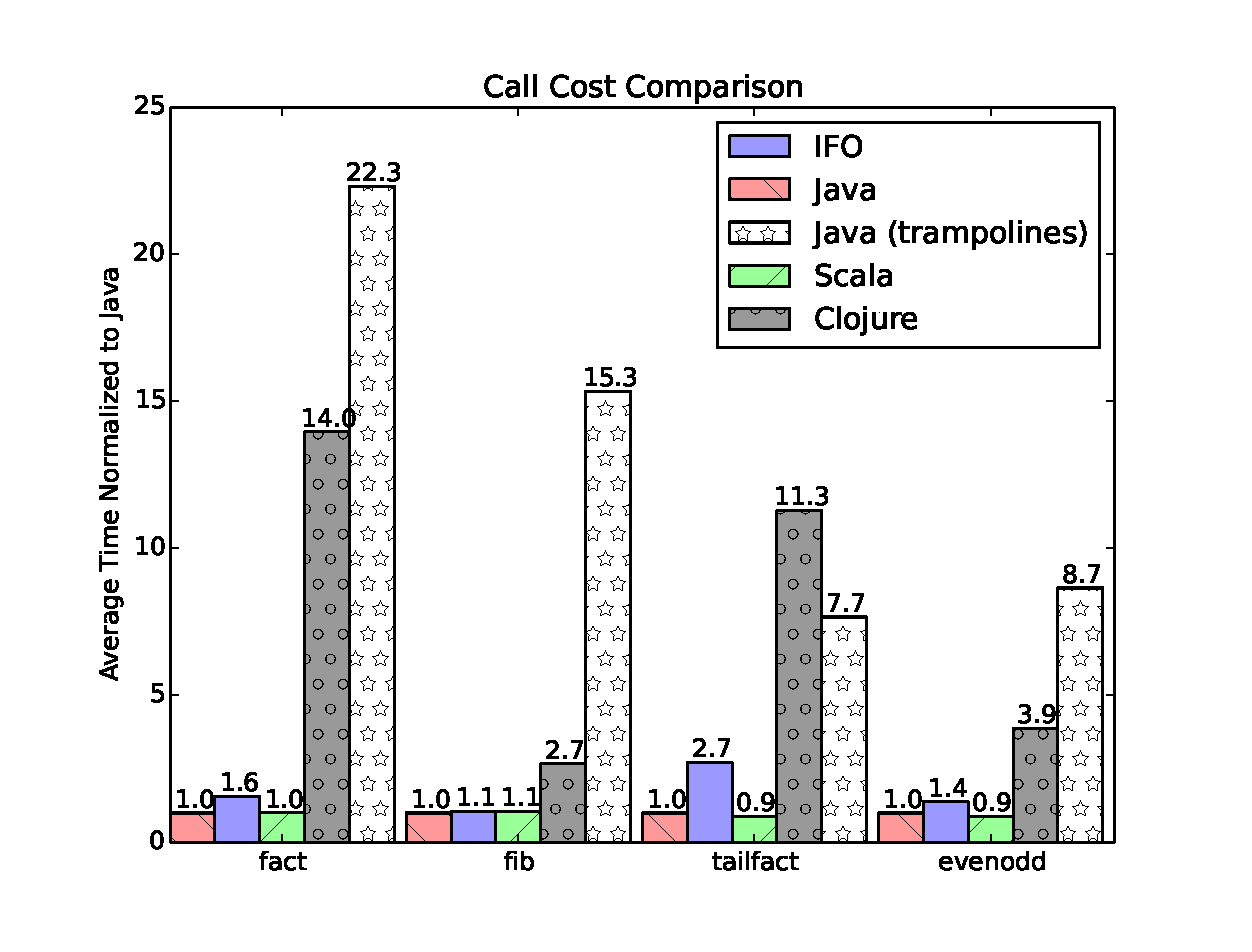
\includegraphics[width=8cm]{./src/img/low.eps}}\end{minipage} &
\begin{minipage}{8cm}{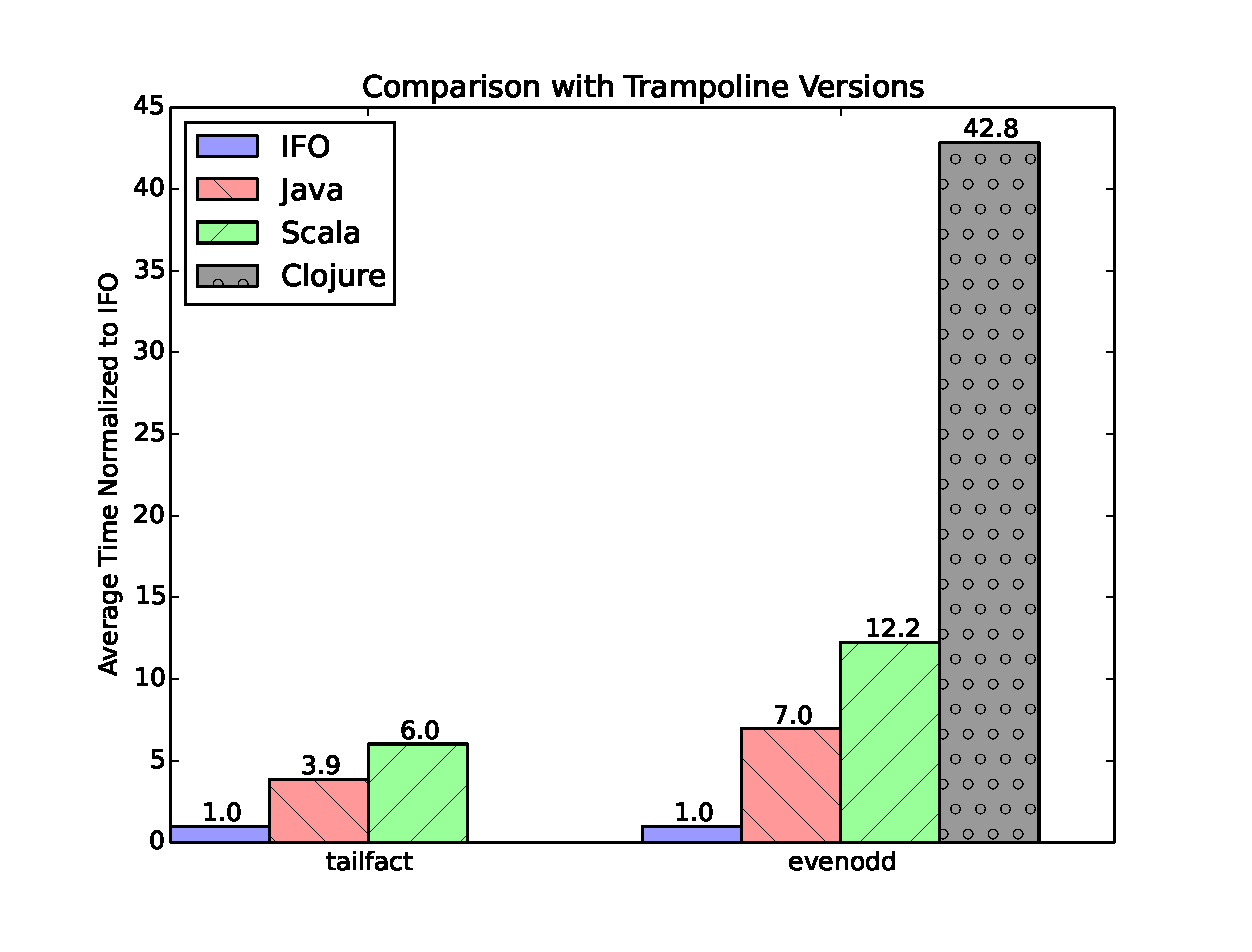
\includegraphics[width=8cm]{./src/img/high.eps}}\end{minipage}
\end{tabular}

\end{center}
\vspace{-20pt}
  \caption{The isolated call behavior experiments: the reported times are averages of 10 measured runs and corresponding standard deviations. The plots are normalized to Java's (left table and plot) and IFO's (right table and plot) results -- the lower, the faster.}

\label{fig:micro}
\end{figure*}

\begin{figure*}[h!t]
\vspace{10pt}
 \begin{center} 
\begin{tabular}{|l|l|l|l|l||l|l|}
\hline
\multicolumn{1}{|r|}{\textit{\textbf{Input length (time unit)}}} & 1000 ($\mu s$)                 & 3000 ($\mu s$)                  & 10000 ($\mu s$)                   & 100000 ($\mu s$)    & Objects (Min) & Objects (Max)               \\ \hline
\textbf{IFO}                                  & $5.10 \pm 0.10$   & $15.98 \pm 0.07$  & $77.81 \pm 0.83$   & $933.58 \pm 13.40$ &  5451 & 5451    \\ \hline
\textbf{Java (Trampoline-based)}                             & $7.03 \pm 0.130$ & $26.89 \pm 0.10$ & $102.98 \pm 2.36$ & $1099.80 \pm 15.46$ & 4665 & 104879\\ \hline
\textbf{Java (Method-based)}                             & $3.80 \pm 0.07$  & $11.61 \pm 0.10$  & $48.83 \pm 0.13$    & N/A  & 4128 & 4128                      \\ \hline
\textbf{Java (FAO-based)}                           & $6.37 \pm 0.01$   & $17.62 \pm 0.05$  & N/A                     & N/A & 18102 & 24082                       \\ \hline
\end{tabular}
  \begin{tabular}{ll}
  \begin{minipage}{8cm}{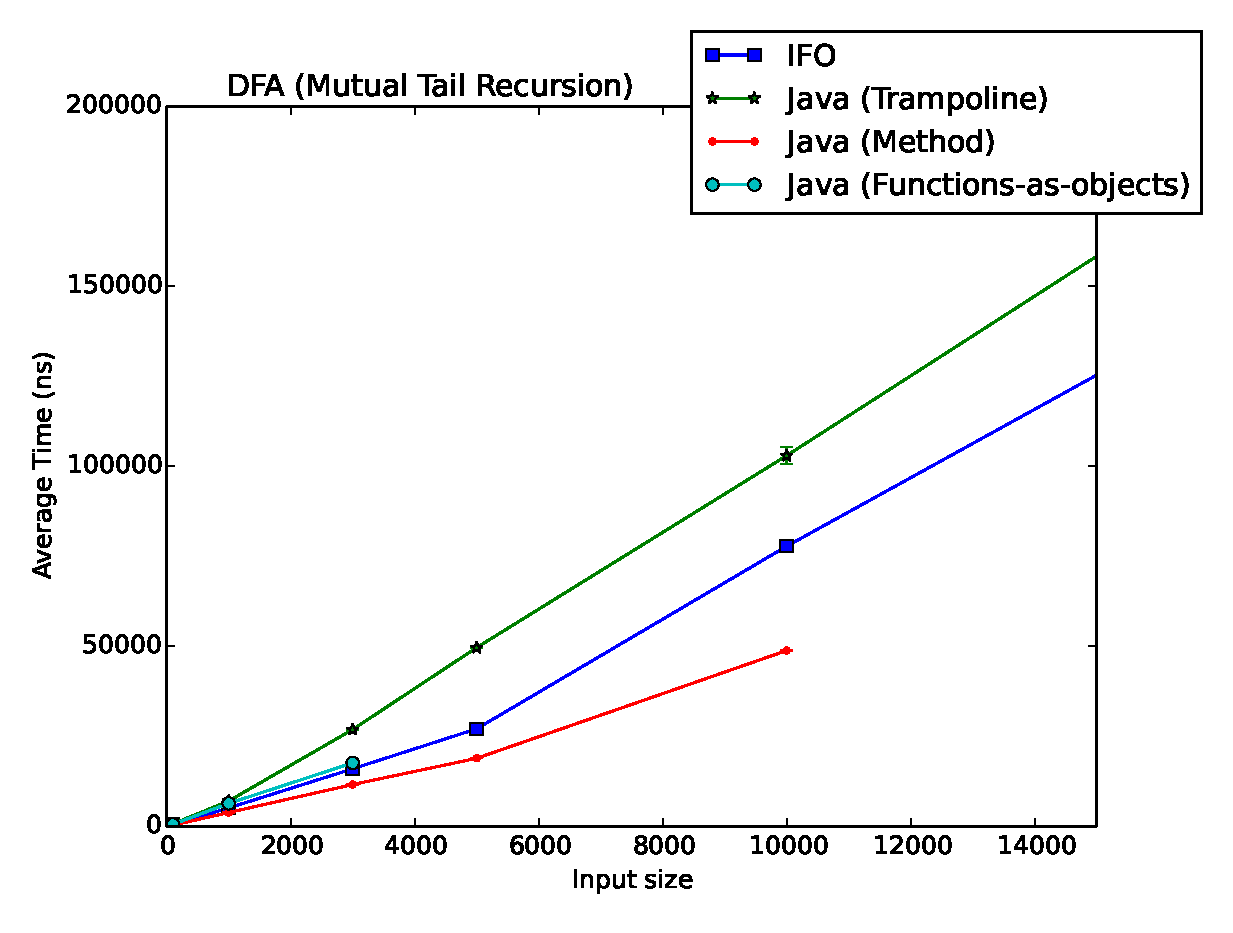
\includegraphics[width=8cm]{./src/img/dfa1.eps}}\end{minipage} &
\begin{minipage}{8cm}{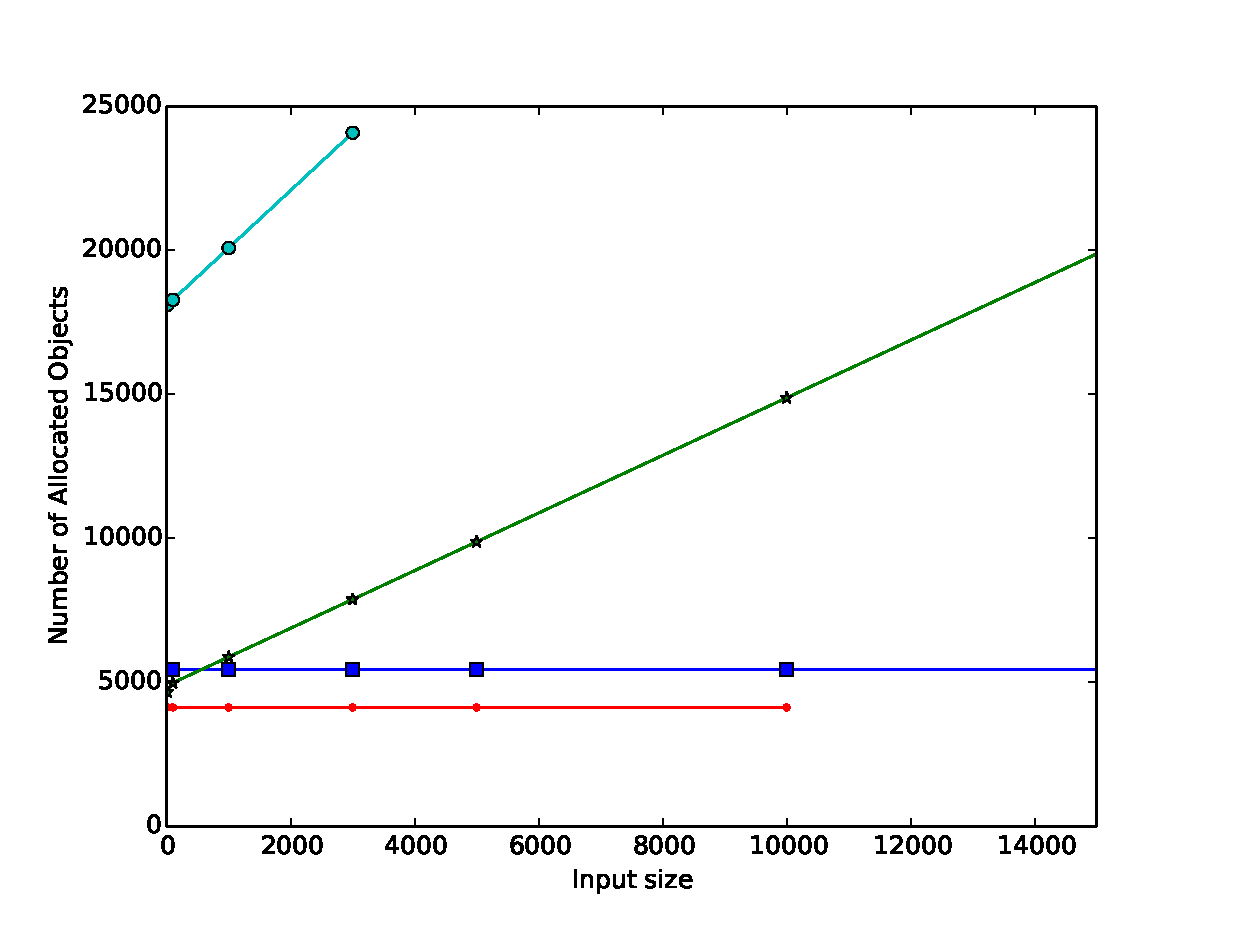
\includegraphics[width=8cm]{./src/img/dfa2.eps}}\end{minipage} 
\end{tabular}

\end{center}
\vspace{-15pt}
\caption{The DFA encoding: the reported times are averages of 10 measured runs and corresponding standard deviations; the last two columns show the minimum and maximum numbers of total allocated objects on heap from isolated profiled runs with all input lengths. Due to space limitations, the x-axes of plots are cropped at 15000 for clarity.}

\label{fig:dfa}
\end{figure*}

\begin{figure*}[h!t]
\vspace{5pt}
 \begin{center} 
\begin{tabular}{|l|l|l|l|l|l|}
\hline
\multicolumn{1}{|r|}{\textit{\textbf{Input length (time units)}}} & 10 ($\mu s$)  & 20 ($\mu s$)   & 40 ($ms$)     & 50 ($ms$)     & 75 ($ms$)     \\ \hline
\textbf{Java (Trampoline-based)}                                       & $17.10 \pm 0.26$ & $320.42 \pm 5.88$ & $14.84 \pm 0.27$ & $62.35 \pm 1.06$ & $1044.61 \pm 12.99$ \\ \hline
\textbf{IFO}                                                      & $11.06 \pm 0.55$ & $289.19 \pm 6.52$ & $12.70 \pm 0.26$ & $48.47 \pm 1.08$ & $805.06 \pm 7.06$ \\ \hline
\textit{Relative speedup}                                         & 54.6\%           & 10.8\%            & 16.9\%           & 28.6\%           & 29.8\%          \\ \hline
\end{tabular}
\end{center}

\vspace{-5pt}
\caption{The 0-1 Knapsack Problem encoded using CPS for different input sizes (the length of weight and value lists) for a fixed total weight of 10: the reported times are averages of 10 measured runs and corresponding standard deviations. 
%Method-based and FAO implementations could not run beyond the input of length 10; their execution times at 10 were $9.68 \pm 0.20~\mu s$ and $13.79 \pm 0.22~\mu s$ respectively.
}

\label{fig:cps}
\end{figure*}

\section{Evaluation}

%Apart from the correctness and uniformity of the representation, 
\name performs well in common FP scenarios. Our evaluation of this claim consists of two
parts. We first compare time performance results of benchmark programs
that isolate different call behaviors. Then, we demonstrate two
application use cases and examine their scalability.

\subsection{Isolated Call Behavior}\label{sec:micro}

In this experiment, we want to evaluate runtime performance of
programs representing different common call behaviors in FP.
We compare the measured average times of these programs
written in \name (to assess IFOs) and of corresponding
programs written in Scala, Clojure, and Java using standard functions
(as methods) and trampolines.

\paragraph{Benchmark Design.}
We wrote the benchmark programs in the extended System F for our
compilation process and in the following JVM-hosted languages in their
latest stable versions:

\begin{itemize}

  \item \emph{Scala} (2.11.2): Scala is one of the most popular
    strongly-typed multi-paradigm languages on the JVM
    \cite{Odersky2014b}. It directly compiles down to the Java
    bytecode and applies various optimizations. In order to encode
    mutually recursive tail calls, we used the provided trampoline
    facility (\texttt{scala.util.control.} \texttt{TailCalls}).

  \item \emph{Clojure} (1.6.0): Clojure is a dynamically-typed,
    functional language which compiles to the Java bytecode
    \cite{Hickey2008}. For mutually recursive tail calls, we used
    \texttt{tramp} from \texttt{clojure.core.} \texttt{logic}.
  
  \item \emph{Java} (1.8.0\_25): We implemented two versions, one
    version using method calls in Java 8 and one using custom
    (hand-written and optimized) trampolines.

\end{itemize}
  
\noindent To evaluate IFOs, we used the \name compiler with all the
optimizations mentioned in Sections \ref{sec:tce} and
\ref{sec:implementation}.

\noindent We executed all benchmarks on the following platform with
the latest Java HotSpot\texttrademark VM (1.8.0\_25):
Intel\textregistered Core\texttrademark i5 3570 CPU, 1600MHz DDR3 4GB
RAM, Ubuntu 14.04.1.
  
\noindent For the automation of performance measurement, we used the
Java Microbenchmark Harness (JMH) tool which is a part of OpenJDK
\cite{jmh}. Based on the provided annotations, JMH measures execution
of given programs. In addition to that, it takes necessary steps to
gain stable results. They include non-measured warm-up iterations for
JITC, forcing garbage collection before each benchmark, and running
benchmarks in isolated VM instances. We configured JMH for 10 warm-up
runs and 10 measured runs from which we compute averages.

\paragraph{Programs.}

We chose four programs to represent the following behaviors:

\begin{itemize}

  \item \emph{Non-tail recursive calls}: Computing the factorial and
    Fibonacci numbers using naive algorithms.

  \item \emph{Single method tail recursive calls}: Computing factorial
    using a tail recursive implementation.

  \item \emph{Mutually recursive tail calls}: Testing evenness and
    oddness using two mutually recursive functions.
\end{itemize}

\noindent Non-tail recursive programs present two examples of general
recursive calls and we executed them, altogether with the tail
recursive programs, on low input values (not causing
\lstinline{StackOverflow} exceptions in default JVM settings). In
addition to that, we executed the tail recursive programs on high input
values in which method-based implementations threw
\lstinline{StackOverflow} exceptions in default JVM settings.
  
\paragraph{Results.}

We show the results in Figure \ref{fig:micro}. Its left part shows
the result for low input values in IFOs, method implementations in all
the other languages and the fastest trampoline implementation (Java);
the plot is normalized to the Java method-based
implementation's results. The right part shows the result for high input values
in IFO- and trampoline-based implementations; the plot is normalized to results of 
IFO-based implementations.

For low input values, we can see that IFO-based implementations run
slightly slower than method-based ones. However, their overhead is
small compared with the fastest trampoline implementations in our
evaluation. IFOs ran 0.1 to 1.7-times slower than method-based
representations, whereas the fastest trampolines ran 7.7 to 22.3-times
slower. In the tail recursive programs, Scala ran slightly faster than
standard Java methods due to its compiler optimizations. Clojure has
an additional overhead, because its compiler enforces integer overflow
checking.

For the high input values, the method-based implementations threw a
\lstinline{StackOverflow} exception in default JVM settings, unlike
IFOs and trampoline implementations which can continue executing with
this input. IFOs ran 3.9 to 12.2-times faster (excluding Clojure) than
trampoline implementations. Again, Clojure suffered from its
additional overhead and threw an integer overflow exception in the
tail recursive factorial. Using BigIntegers would prevent this, but
we wanted to isolate the call behavior in this experiment, i.e. avoid
any extra overhead from other object allocations.

\subsection{Applications}

In this experiment, we examine the time and memory scalability of IFOs
and alternative closure representations (methods,
functions-as-objects, and trampolines) in two applications which
make use of tail calls. Unlike Section \ref{sec:micro}, where
the programs isolated costs of plain recursive calls, the applications
here represent a more realistic behavior with other costs, such as
non-recursive method calls, calls to other API methods or partial applications.

We implemented the applications in \name to assess
IFOs and in Java to assess different closure representations: method
calls, Java 8's lambdas (functions-as-objects), and custom
trampolines. We chose Java, because our custom implementation of
trampolines performed best in the isolated call behavior
experiments. Using plain Java implementations, we can examine the
runtime behavior of different representations without potential
compiler overheads.  We performed the time measurement in the same
setting as in the previous experiment. For the memory, we report the
total number of allocated objects on heap in the isolated application
runs, as measured by HPROF~ \cite{hprof}, the JDK's profiling tool.

\paragraph{DFA Encoding.}\label{sec:dfa}

One common idiom in functional programming is encoding finite states
as tail recursive functions and state transitions as mutual calls
among these functions. One trivial example of this is the naive
even-odd program which switches between two states. A more useful
application is in the implementation of finite state automata
\cite{Krishnamurthi2006}. Normally, functional language programmers
seek this idiom for its conciseness. However in JVM-hosted functional
languages, programmers tend to avoid this idiom, because they either
lose correctness (\lstinline{StackOverflow} exceptions in a
method-based representation) or performance (in a trampoline-based
one). In this experiment, we implemented a DFA recognizing a regular
expression $(AAB^{*}|A^{*}B)^{+}$ and measured the performance on
randomly generated Strings with different lengths.

We show the result of this experiment in Figure \ref{fig:dfa}. The
FAO-based implementation ran slowest out of all implementations and threw
\lstinline{StackOverflow} exception with a smaller input than the
method-based implementation. That is because it creates extra objects
and performs extra calls due to its representation. As in the isolated
calls experiment, the IFO-based implementation ran about 0.5-times slower than method-based
implementation. Trampolines, however, ran about 2-times slower. The IFO-
and trampoline-based implementations continued executing after method-based
one threw a \lstinline{StackOverflow} exception. The IFO-based
implementation was about 0.2-times faster than the trampoline one for 
larger inputs.

What is more important here is the memory consumption. IFOs, similarly
to the method-based implementation, allocated a constant number of
objects on heap. The trampoline one, however, increased its object
allocation with the input, because it needed to create an object for 
each tail call.

\paragraph{CPS Encoding of Knapsack.}\label{sec:cps}

Tail calls find their application in continuation-passing style
\cite{Steele1975} where each call is a tail call.  In this
application, we encoded a naive implementation of the 0-1 Knapsack
Problem with multiple recursive calls and also non-recursive tail
calls.  In the experiment, we fixed the total weight to 10 and
generated input values and weights lists of different sizes: we
generated weights as consecutive sequences 1 to 5 and values as
$i\times weight[i]$.

We show the results in Figure \ref{fig:cps}. This implementation contains 
partial applications and a pure method-based implementation is impossible in this style.
The method- and FAO-based implementations could not run beyond the input of length 10 due to a \lstinline{StackOverflow} exception; their execution times at 10 were $9.68 \pm 0.20~\mu s$ and $13.79 \pm 0.22~\mu s$ respectively. IFOs ran 10.8\% to 54.6\% faster than the trampoline implementation in different input lengths.

\subsection{Discussion}

The programs benchmarked in Section \ref{sec:micro} stressed the time
spent on recursive calls. These programs are quite simple, but
representative of common patterns of functional programming. IFOs gave
a 3.9 to 12.2-times speed-up over the trampoline implementations. This
huge gain is also due to other optimizations in our compiler. In
particular, since those programs have small and simple definitions,
inlining is beneficial and gives a big performance gain on top of the
gains for TCE. In the more complex scenarios of Section
\ref{sec:dfa}, the tail calls are not the only runtime cost, so the
overhead of trampolines is much smaller. Still, IFO programs gained a
speed-up of 0.1 to 0.5 over our hand-written and optimized
trampolines.  The other benefit for programs with tail recursion
is the constant memory overhead of calls in IFOs.
This also appears in method-based implementations, but they
throw a \lstinline{StackOverflow} exception in larger inputs and IFOs
do not.



\section{Related Work}

This section discusses related work: intermediate functional languages on top of the JVM,
TCE and function representations, TCE on the JVM, and the JVM modifications.

\paragraph{Intermediate Functional Languages on top of the JVM.}
A primary objective of our work is to create an efficient intermediate
language that targets the JVM. With such intermediate language,
compiler writers can easily develop FP compilers in the JVM.
System F is an obvious candidate for an intermediate language as it
serves as a foundation for ML-style or Haskell-style FP languages.
However, there is no efficient implementation of System F in the JVM.
The only implementation of System F that we know of (for a JVM-like
platform) was done by Kennedy and Syme~\cite{Kennedy2004}. They showed
that System F can be encoded, in a type-preserving way, into
.NET's C\#. That encoding could easily be employed in Java or the JVM as
well. However, their focus was different from ours. They were not aiming
at having an efficient implementation of System F. Instead, their goal
was to show that the type system of languages such as C\# or Java is
expressive enough to faithfully encode System F terms. They used a
FAO-based approach and have not exploited the erasure semantics of System F.
As a result, the encoding suffers from various performance drawbacks
and cannot be realistically used as an intermediate language. MLj
\cite{Benton1998} compiled a subset of SML '97 (interoperable with
Java libraries) to the Monadic Intermediate Language, from which it
generated Java bytecode. Various Haskell-to-JVM compiler backends
\cite{Wakeling1999,Tullsen1996,Choi2001} used different
variations of the \emph{graph reduction machine}~\cite{Wadsworth:1971} for their
code generation, whereas we translate from System F. 

\paragraph{Tail-Call Elimination and Function Representations.}
A choice of a function representation plays a great role
\cite{Shao1994} in time and space efficiency as well as in how
difficult it is to correctly implement tail calls. Since
Steele's pioneering work on tail calls \cite{Steele1977}, implementors
of FP languages often recognize TCE as a necessary
feature. Steele's Rabbit Scheme compiler~\cite{Steele1978} introduced the ``UUO handler'' 
that inspired our TCE technique using IFOs.
Early on, some Scheme compilers targeted C as an intermediate
language and overcame the absence of TCE in the backend compiler by
using trampolines. Trampolines incur on performance penalties and
different techniques, with ``Cheney on the M.T.A." \cite{Baker1995}
being the most known one, improved upon them. The limitations of the
JVM architecture, such as the lack of control over the memory
allocation process, prevent a full implementation of Baker's
technique. 

\paragraph{Tail-Call Elimination on the JVM.}
Apart from the recent languages, such as Scala \cite{Odersky2014b} or
Clojure \cite{Hickey2008}, functional languages have
targeted the JVM since its early versions. 
Several other JVM functional languages support (self) tail recursion
optimization, but not full TCE. Examples include MLj \cite{Benton1998}
or Frege~\cite{Wechsung}.  Later work \cite{Minamide2003} extended MLj
with Selective TCE. This work used an effect system to estimate the number
of successive tail calls and introduced trampolines only when
necessary. Another approach to TCE in the JVM  is to 
use an explicit stack on the heap (an \texttt{Object[]} array)~\cite{Choi2001}. 
With such explicit stack for TCE, the approach from Steele's pioneering work \cite{Steele1978} 
can also be encoded in the JVM. Our work avoids the need for an explicit stack by using 
IFOs, thus allowing for a more direct implementation of this technique. 
The Funnel compiler for the JVM \cite{Schinz2001} used
standard method calls and shrank the stack only after the execution
reached a predefined ``tail call limit". This dynamic optimization
needs careful tuning of the parameters, but can be possibly used to
further improve performance of our approach.

\paragraph{JVM Modifications.}
Proposals to modify the JVM \cite{League2001}, which would arguably be a better
solution for improving support for FP,
appeared early on. One reason why the JVM does not support tail calls
was due to a claimed incompatibility of a security mechanism based on
stack inspection with a global TCE policy. The abstract
continuation-marks machine \cite{Clements2004} refuted this
claim. There exists one modified Java HotSpot\texttrademark VM
\cite{Schwaighofer2009} with TCE support. The research Maxine VM
with its new self-optimizing runtime system \cite{Wuerthinger2013}
allows a more efficient execution of JVM-hosted languages. Despite
these and other proposals and JVM implementations, such as IBM J9, we
are not aware of any concrete plans for adding TCE support to the
next official JVM release. Some other virtual machines designed for
imperative languages do not support TCE either. For example, the
standard Python interpreter lacks it, even though some enhanced
variants can overcome this issue \cite{Tismer2000}. Hence, ideas from our
work can be applied outside of the JVM ecosystem.


\section{Conclusion \& Future Work}\label{sec:conclusion}
Functional Programming in the JVM is already possible today. 
However, when efficiency is a concern, programmers and compiler 
writers still need to be aware of the limitations of the JVM. 
Some of the problems are the need for two function representations; 
and the lack of a good solution for TCE. This paper shows that IFOs allow for a uniform representation of 
functions, while being competitive in terms of time performance and 
supporting TCE in constant space.

There is much to be done for future work. We would like to prove
correctness results for our translation from System F to Java. To
achieve this, we will first need a suitable formalization of Java that
includes inner classes and imperative features. Furthermore, we
will adopt the thread-safe version of our translation -- one main difference is that
IFOs should be allocated at their call sites rather than at their definition sites.
  One other aspect is with currying and partial applications,
where the uniform function representation is important.
FAOs here can have substantial time and memory overheads, especially when defining multi-argument
recursive functions, so current languages tend to avoid them and use two representations:
JVM methods when possible; and FAOs when necessary.
With additional optimizations in \Name, such as multi-argument closure optimization
and unboxing, IFOs serve as one uniform efficient function representation.
 We would like to formalize and refine a number of optimizations that we
have been experimenting with in \Name; and explore what other optimizations are possible
with IFOs.
Finally, we want to build frontends for
realistic functional languages on top of \name and write large
functional programs, including a full bootstrapping compiler of \Name, in those frontends.



\subsubsection*{Acknowledgments.}
We would like to thank T. H. Tse, C.-L. Wang, Vlad Urechte, R\'{u}nar Bjarnason, and \name contributors for help and valuable feedback on previous drafts of this work. We also thank the anonymous reviewers for their helpful suggestions. The work described in this paper was partially supported by a grant from the Research Grants Council of the Hong Kong Special Administrative Region, China (Project No. HKU 27200514).

% Bibliography
\bibliographystyle{splncs}
\bibliography{papers}

\end{document}
